%
% Copyright 2018 Joel Feldman, Andrew Rechnitzer and Elyse Yeager.
% This work is licensed under a Creative Commons Attribution-NonCommercial-ShareAlike 4.0 International License.
% https://creativecommons.org/licenses/by-nc-sa/4.0/
%
\questionheader{ex:s2.4}

\noindent
Recall that we are using $\log x$ to denote the logarithm of $x$ with
base $e$. In other courses it is often denoted $\ln x$.

%%%%%%%%%%%%%%%%%%
\subsection*{\Conceptual}
%%%%%%%%%%%%%%%%%%

\begin{Mquestion}
Below are pairs of functions $y=f(x)$ and differential equations. For each pair, decide whether the function is a solution of the differential equation.
\begin{center}
\begin{tabular}{c| l | l|}
\cline{2-3}
~&\textbf{function}&\textbf{differential equation}\\
\cline{2-3}
(a)&$y=5(e^x-3x^2-6x-6)$&$\displaystyle \diff{y}{x}=y+15x^2$\\
(b) & $y=\dfrac{-2}{x^2+1}$&$y'(x)=xy^2$\\
(c)&$y=x^{3/2}+x$&$\displaystyle\left(\diff{y}{x}\right)^2 + \diff{y}{x}=y$\\
\cline{2-3}
\end{tabular}
\end{center}
\end{Mquestion}
\begin{hint}
You don't need to solve the differential equation from scratch, only verify whether the given function $y=f(x)$ makes it true. Find $\diff{y}{x}$ and plug it into the differential equation.
\end{hint}
\begin{answer}
(a) yes \qquad (b) yes \qquad (c) no
\end{answer}
\begin{solution}
\begin{enumerate}[(a)]
\item If $y=5(e^x-3x^2-6x-6)$, then $\diff{y}{x} = 5(e^x-6x-6)$. Let's see whether this is equal to $y+15x^2$:
\begin{align*}
y+15x^2&=5(e^x-3x^2-6x-6)+15x^2\\
&=5(e^x-3x^2-6x-6+3x^2)\\
&=5(e^x-6x-6)\\
&=\diff{y}{x}
\end{align*}
So, $y=5(e^x-3x^2-6x-6)$ is indeed a solution to the differential equation $\diff{y}{x}=y+15x^2$.
%
\item If $y=\dfrac{-2}{x^2+1}$, then  $\diff{y}{x} = \dfrac{4x}{(x+1)^2}$. Let's see whether this is equal to $xy^2$:
\begin{align*}
xy^2&=x\left(\frac{-2}{x^2+1}\right)^2\\
&=\frac{4x}{(x^2+1)^2}\\
&=\diff{y}{x}
\end{align*}
So, $y=\dfrac{-2}{x^2+1}$ is indeed a solution to the differential equation $\diff{y}{x}=yx^2$.
%
\item If $y=x^{3/2}+x$, then  $\diff{y}{x} = \frac{3}{2}\sqrt{x}+1$.
\begin{align*}
\left(\diff{y}{x}\right)^2+\diff{y}{x}&=\left(\frac{3}{2}\sqrt{x}+1\right)^2+\frac{3}{2}\sqrt{x}+1\\
&=\frac{9}{4}x+\frac{9}{2}\sqrt{x}+2\\
&\neq \diff{y}{x}
\end{align*}
So, $y=x^{3/2}+x$ is not a solution to the differential equation $\left(\diff{y}{x}\right)^2+\diff{y}{x}=y$.
\end{enumerate}
\end{solution}

%%%%%%%%%%%%%%%%%%%
\begin{Mquestion}
Following Definition~\eref{CLP101}{def:SDEsepdiffeq} in the CLP-2 text, a separable differential equation has the form
\[\diff{y}{x}(x) = f(x)\ g\big(y(x)\big).\]
Show that each of the following equations can be written in this form, identifying $f(x)$ and $g(y)$.
\begin{enumerate}[(a)]
\item $3y\diff{y}{x}=x\sin y$
\item $\diff{y}{x} = e^{x+y}$
\item  $\diff{y}{x}+1=x$
\item $\left(\diff{y}{x}\right)^2-2x\diff{y}{x}+x^2=0$
\end{enumerate}
\end{Mquestion}
\begin{hint}
For (d), note the equation given is quadratic in the variable $\diff{y}{x}$.
\end{hint}
\begin{answer}
\begin{enumerate}[(a)]
\item One possible answer: $f(x)=x$, $g(y)=\dfrac{\sin y}{3y}$.
\item One possible answer:  $f(x) = e^x$, $g(y) = e^y$.
\item One possible answer:  $f(x) = x-1$, $g(y) = 1$.
\item The given equation is equivalent to the equation $\diff{y}{x}=x$, which fits the form of a separable equation with $f(x)=x$, $g(y)=1$.
\end{enumerate}
\end{answer}
\begin{solution}
\begin{enumerate}[(a)]
\item $3y\diff{y}{x}=x\sin y$ can be written as $\diff{y}{x} = x\left(\frac{\sin y}{3y}\right)$, which fits the form of a separable equation with $f(x)=x$, $g(y) = \frac{\sin y}{3y}$.
\item $\diff{y}{x} = e^{x+y} = e^xe^y$
which fits the form of a separable equation using $f(x) = e^x$, $g(y) = e^y$.
\item  $\diff{y}{x}+1=x$ can be written as $\diff{y}{x} = (x-1)$, which fits the form of a separable equation using $f(x)=x-1$, $g(y)=1$. (We can solve it by simply antidifferentiating.)
\item Notice the left side of the equation $\left(\diff{y}{x}\right)^2-2x\diff{y}{x}+x^2=0$ is a perfect square. So, this equation is equivalent to $\left(\diff{y}{x}-x\right)^2=0$, that is, $\diff{y}{x}=x$. This has the form of a separable equation with $f(x)=x$, $g(y)=1$.
\end{enumerate}
\end{solution}

%%%%%%%%%%%%%%%%%%
\begin{question}
Suppose we have the following functions:
\begin{itemize}
\item $y$ is a differentiable function of $x$
\item $f$ is a function of $x$, with $\int f(x)\,\dee{x}=F(x)$
\item $g$ is a nonzero function of $y$, with $\int \frac{1}{g(y)} \,\dee{y}=G(y)=G(y(x))$.
\end{itemize}

In the work below, we set up a solution to the separable differential equation
\[\diff{y}{x}=f(x)g(y)=f(x)g(y(x)))\]
without using the mnemonic of Equation~\eref{CLP101}{eq:SDEbasicSln} in the CLP-2 text.

By deleting some portion of our work, we can create the solution as it would look using the mnemonic. What portion can be deleted?

Remark: the purpose of this exercise is to illuminate what, exactly, the mnemonic is a shortcut for. Despite its peculiar look, it agrees with what we already know about integration.

\begin{quote}
\color{blue}
\begin{align*}
\diff{y}{x}&=f(x)g(y(x))
\intertext{Since $g(y(x))$ is a nonzero function, we can divide both sides by it.}
\frac{1}{g(y(x))}\cdot\diff{y}{x}&=f(x)
\intertext{If these functions of $x$ are the same, then they have the same antiderivative with respect to $x$.}
\int \frac{1}{g(y(x))}\cdot\diff{y}{x}\,\dee{x}&=\int f(x)\,\dee{x}
\intertext{The left integral is in the correct form for a change of variables to $y$. To make this easier to see, we'll use a $u$-substitution, since it's a little more familiar than a $y$-substitution. If $u=y$, then $\diff{u}{x}=\diff{y}{x}$, so $\dee{u}=\diff{y}{x}\dee{x}$.}
\int\frac{1}{g(u)}\,\dee{u}&=\int f(x)\,\dee{x}
\intertext{Since $u$ was just the same as $y$, again for cosmetic reasons, we can swap it back. (Formally, you could have skipped the step above--we just included it to be extra clear that we're not using any integration techniques we haven't seen before.)}
\int\frac{1}{g(y)}\,\dee{y}&=\int f(x)\,\dee{x}
\intertext{We're given the antiderivatives in question.}
G(y)+C_1&=F(x)+C_2\\
G(y)&=F(x)+(C_2-C_1)
\intertext{where $C_1$ and $C_2$ are arbitrary constants. Then also $C_2-C_1$ is an arbitrary constant, so we might as well call it $C$.}
G(y)&=F(x)+C
\end{align*}
\end{quote}
\end{question}
\begin{hint}
The step $\displaystyle\int \frac{1}{g(y)}\,\dee{y} = \int f(x)\,\dee{x}$ shows up whether we're using our mnemonic or not.
\end{hint}
\begin{answer}
The mnemonic allows us to skip from the separable differential equation we want to solve (very first line) to the equation
\[\int \frac{1}{g(y)}\,\dee{y}=\int f(x)\,\dee{x}\]
\end{answer}
\begin{solution}
The mnemonic allows us to skip from the separable differential equation we want to solve (very first line) to the equation
\[\int \frac{1}{g(y)}\,\dee{y}=\int f(x)\,\dee{x}\]
So, the mnemonic is just a shortcut for the substitution we performed to get this point.

We also generally skip the explanation about $C_1$ and $C_2$ being replaced with $C$.
\end{solution}

%%%%%%%%%%%%%%%%%%
\begin{Mquestion}
Suppose $y=f(x)$ is a solution to the differential equation $\diff{y}{x}=xy$.

True or false: $f(x)+C$ is also a solution, for any constant $C$.
\end{Mquestion}
\begin{hint}
Note $\diff{}{x}\{f(x)\} = \diff{}{x}\{f(x)+C\}$. Plug in $y=f(x)+C$ to the equation
 $\diff{y}{x}=xy$ to see whether it makes the equation is true.
\end{hint}
\begin{answer}
false
\end{answer}
\begin{solution}
To say $y=f(x)+C$ is a solution to the differential equation means:
\begin{align*}
\diff{}{x}\{f(x)+C\}&=x(f(x)+C)
\intertext{Since $y=f(x)$ is a solution, we know $\diff{}{x}\{f(x)\}=xf(x)$. Also, $\diff{}{x}\{f(x)+C\}=\diff{}{x}\{f(x)\}$. So, $\diff{}{x}\{f(x)+C\}=xf(x)$.}
xf(x)&=x(f(x)+C)\\
0&=xC
\end{align*}
Our equation should hold for all $x$ in our domain, and for the derivative to $y$ with respect to $x$ to make sense, our domain should not be a single point. So, there is some $x$ in our domain such that $x \neq 0$. Therefore, the  $C$ \emph{must be zero}. So, $f(x)+C$ is \emph{not} a solution to the differential equation for any constant $C$.

When we're finding a general antiderivative, we add ``$+C$" at the end. When we're finding a general solution to a differential equation, the ``$+C$" gets added when we antidifferentiate--we don't add another one at the end of our work.
\end{solution}




%%%%%%%%%%%%%%%%%%
\begin{question}
Suppose a function $y=f(x)$ satisfies $|y| = Cx$, for some constant $C>0$.
\begin{enumerate}[(a)]
\item What is the largest possible domain of $f(x)$, given the information at hand?
\item Give an example of function $y=f(x)$  with the following properties, or show that none exists:
\begin{itemize}
\item $|y| = Cx$,
\item $\diff{y}{x}$ exists for all $x>0$, and
\item $y>0$ for some values of $x$, and $y<0$ for others.
\end{itemize}
\end{enumerate}
\end{question}
\begin{hint}
If a function is differentiable at a point, it is also continuous at that point.
\end{hint}
\begin{answer}
(a) $[0,\infty)$\\
(b) No such function exists. If $|f(x)|=Cx$ and $f(x)$ switches from $f(x)=Cx$ to $f(x)=-Cx$ at some point, then that point is a jump discontinuity. Where $f(x)$ contains a discontinuity, $\diff{y}{x}$ does not exist.
\end{answer}
\begin{solution}
\begin{enumerate}[(a)]
\item Since $|y| \geq 0$ no matter what $y$ is, we see $Cx \ge 0$ for all $x$ in the domain of $f(x)$. Since $C$ is positive, that means the domain of $f(x)$ only includes nonnegative numbers. So, the largest possible domain of $f(x)$ is $[0,\infty)$.
\item None exists.

The graph of $Cx$ is given below for some positive constant $C$, also with the graph of $-Cx$. If $y=f(x)$ were sometimes the top function, and other times the bottom function, then there would be a jump discontinuity where it switched. Then the derivative of $f(x)$ would not exist, violating the second property.
\begin{center}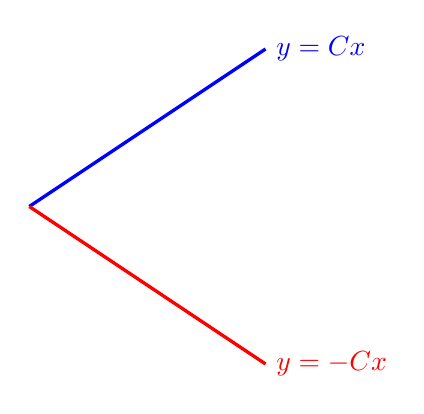
\begin{tikzpicture}
\YEaaxis{.5}{3.5}{2.5}{2.5}
\draw[very thick, blue] (0,0)--(3,2) node[right]{$y=Cx$};
\draw[very thick, red] (0,0)--(3,-2) node[right]{$y=-Cx$};
\end{tikzpicture}\end{center}

A tiny technical note is that it's possible that $f(x)=Cx$ when $x=0$ and $f(x)=-Cx$ when $x>0$ (or vice-versa). This would not introduce a jump discontinuity, but it also does not satisfy that $f(x)>0$ for some values of $x$.
\end{enumerate}
Remark: in several instances below, solving a differential equation will lead us to conclude something like $|y|=g(x)$. In these cases, we choose either $y=g(x)$, or $y=-g(x)$, but not $y=\pm g(x)$ (which is not a function) or that $y$ is sometimes $g(x)$, and other times $-g(x)$. The reasoning above somewhat explains this choice: if $y$ were sometimes positive and sometimes negative, then $\diff{y}{x}$ would not exist at the values of $x$ where the sign of $y$ switches, unless that switch occurrs at a root of $g(x)$. Since that's a pretty specific occurrence, we usually feel safe ignoring it to avoid getting bogged down in technical details.
\end{solution}




%%%%%%%%%%%%%%%%%%

\begin{question}
Express the following sentence\footnote{The sentence is paraphrased from
the Pharmakokinetics website of  Universit\'e de Lausanne,
``Elimination Kinetics," at \url{https://sepia.unil.ch/pharmacology/index.php?id=94}\,.
The half-life of morphine is given on the same website at \url{https://sepia.unil.ch/pharmacology/index.php?id=85}\ .
Accessed 12 August 2017.} as a differential equation. You don't have to solve the equation.
\begin{quote}
\color{blue}
%About 25 percent of the total quantity of morphine in the bloodstream is eliminated every hour.
About 0.3 percent of the total quantity of morphine in the bloodstream is eliminated every minute.
\end{quote}
\end{question}
\begin{hint}
Let $Q(t)$ be the quantity of morphine in a patient's bloodstream at time $t$, where $t$ is measured in minutes.

Using the definition of a derivative,
\[\diff{Q}{t}=\lim_{h \to 0}\frac{Q(t+h)-Q(t)}{h}\approx \frac{Q(t+1)-Q(t)}{1}\]
So, $\diff{Q}{t}$ is roughly the change in the amount of morphine in one minute, from $t$ to $t+1$.
\end{hint}
\begin{answer}
$\displaystyle \diff{Q}{t}=-0.003Q(t)$
\end{answer}
\begin{solution}
Let $Q(t)$ be the quantity of morphine in a patient's bloodstream at time $t$, where $t$ is measured in minutes.

Using the definition of a derivative,
\[\diff{Q}{t}=\lim_{h \to 0}\frac{Q(t+h)-Q(t)}{h}\approx \frac{Q(t+1)-Q(t)}{1}\]
So, $\diff{Q}{t}$ is roughly the change in the amount of morphine in one minute, from $t$ to $t+1$.

The sentence tells us that the change in the amount of morphine in one minute is about $-0.003Q$, where $Q$ is the quantity in the bloodstream. That is:
\[\diff{Q}{t}=-0.003Q(t)\]
\end{solution}
%%%%%%%%%%%%%%%%%%%

\begin{Mquestion}
Suppose a particular change is occurring in a language, from an old form to a new form.\footnote{
An example is the change in German from ``wollt" to ``wollst" for the second-person conjugation of the verb ``wollen." This example
is provided by the site Laws in Quantitative Linguistics, ``Change in Language" \url{http://lql.uni-trier.de/index.php/Change_in_language} accessed 18 August 2017.
}
 Let $p(t)$ be the proportion (measured as a number between 0, meaning none, and 1, meaning all) of the time that speakers use the new form. Piotrowski's law\footnote{Piotrowski's law is paraphrased from the page \textbf{Piotrowski-Gesetz} on Glottopedia, \url{http://www.glottopedia.org/index.php/Piotrowski-Gesetz}, accessed 18 August 2017. According to this source, the law was based on work by the married couple R. G. Piotrowski and A. A. Piotrowskaja, later generalized by G. Altmann.
} predicts the following.
\begin{quote}\color{blue}
Use of the new form over time spreads at a rate that is proportional to the product of the proportion of the new form and the proportion of the old form.
\end{quote}

Express this as a differential equation. You do not need to solve the differential equation.
\end{Mquestion}
\begin{hint}
If $p(t)$ is the proportion of the new form, then $1-p(t)$ is the proportion of the old form.

When we say two quantities are proportional, we mean that one is a constant multiple of the other.
\end{hint}
\begin{answer}
$\diff{p}{t}=\alpha p(t)\big(1-p(t)\big)$, for some constant $\alpha$.
\end{answer}
\begin{solution}
If $p(t)$ is the proportion of times speakers use the new form, measured between 0 and 1, then $1-p(t)$ is the proportion of times speakers use the old form.

The law, then, states that $\diff{p}{t}$ is proportional to $p(t)\times \big(1-p(t)\big)$. When we say two quantities are proportional, we mean that one is a constant multiple of the other. So, the law says
\[\diff{p}{t}=\alpha p(t)\big(1-p(t)\big)\]
for some constant $\alpha$.

Remark: it follows from this model that, when a new form is either very rare or entirely ubiquitous, the rate of change of its adoption is small. This makes sense: if the new form is used all the time ($p(t)\approx 1$), there's nobody left to convert; if the new form is almost never used ($p(t)\approx 0$) then people don't know about it, so they won't pick it up.
\end{solution}
%%%%%%%%%%%%%%%%%%%
\begin{Mquestion}\label{prob_s2.4:field}
Consider the differential equation $y'=\frac{y}{2}-1$.
\begin{enumerate}[(a)]
\item When $y=0$, what is $y'$?
\item When $y=2$, what is $y'$?
\item When $y=3$, what is $y'$?
\item\label{prob_s2.4:fieldd} On the axes below, interpret the marks we have made, and use them to sketch a possible solution to the differential equation.
\end{enumerate}
\begin{center}
\begin{tikzpicture}
\YEaaxis{.5}{6.5}{3.5}{3.5}
\draw[dotted, gray] (0,-3) grid (6,3);
\YExcoord{1}{1}
\YEycoord{1}{1}
\foreach \x in {0,...,6}{
	\foreach \y in {-3,...,3}{
	\DIVIDE{\y}{2}{\M}
	\SUBTRACT{\M}{1}{\m}
		\draw[rotate around={{atan(\m)}:(\x,\y)},red] (\x-.25,\y)--(\x+.25,\y);}}
\end{tikzpicture}
\end{center}
\end{Mquestion}
\begin{hint}
The red marks show the slope $y(x)$ would have at a point \emph{if} it crosses that point. So, pick a value of $y(0)$; based on the red marks, you can see how fast $y(x)$ is increasing or decreasing at that point, which leads you roughly to a value of $y(1)$; again, the red marks tell you how fast $y(x)$ is increasing or decreasing, which leads you to a value of $y(2)$, etc (unless you're already off the graph).
\end{hint}
\begin{answer}
(a) $-1$ \qquad (b) $0$ \qquad (c) $0.5$\\
(d) Two possible answers are shown below:
\begin{center}
\begin{tikzpicture}
\YEaaxis{.5}{6.5}{3.5}{3.5}
\draw[dotted, gray] (0,-3) grid (6,3);
\YExcoord{1}{1}
\YEycoord{1}{1}
\foreach \x in {0,...,6}{
	\foreach \y in {-3,...,3}{
	\DIVIDE{\y}{2}{\M}
	\SUBTRACT{\M}{1}{\m}
		\draw[rotate around={{atan(\m)}:(\x,\y)},red] (\x-.25,\y)--(\x+.25,\y);}}
\color{blue} \draw[thick] plot[domain=0:2](\x,{-2*(exp(\x/2))+2});
\end{tikzpicture}\hfill
\begin{tikzpicture}
\YEaaxis{.5}{6.5}{3.5}{3.5}
\draw[dotted, gray] (0,-3) grid (6,3);
\YExcoord{1}{1}
\YEycoord{1}{1}
\foreach \x in {0,...,6}{
	\foreach \y in {-3,...,3}{
	\DIVIDE{\y}{2}{\M}
	\SUBTRACT{\M}{1}{\m}
		\draw[rotate around={{atan(\m)}:(\x,\y)},red] (\x-.25,\y)--(\x+.25,\y);}}
\color{blue} \draw[thick] plot[domain=0:1](\x,{(exp(\x/2))+2});
\end{tikzpicture}
\end{center}
Another possible answer is the constant function $y=2$.
\end{answer}
\begin{solution}
\begin{enumerate}[(a)]
\item When $y=0$, $y'=\frac{0}{2}-1=-1$.
\item When $y=2$, $y'=\frac{2}{2}-1=0$.
\item When $y=3$, $y'=\frac{3}{2}-1=0.5$.
\item The small red lines have varying slopes. The red lines on points with $y$-coordinate 2 have slopes of  $0$; this matches $y'$ when $y=0$, as we saw above.
The red lines on points with $y$-coordinate 0 have slopes of approximately $-1$;
again, this matches what we found for $y'$ when $y=0$.

The red lines correspond to a tiny section of $y(x)$, \emph{if} $y(x)$ passes through that point. So, we can sketch a possible curve $y(x)$ satisfying the equation by starting somewhere, then following the slopes.

For example, suppose we start at the origin.
\begin{center}
\begin{tikzpicture}
\YEaaxis{.5}{6.5}{3.5}{3.5}
\draw[dotted, gray] (0,-3) grid (6,3);
\YExcoord{1}{1}
\YEycoord{1}{1}
\foreach \x in {0,...,6}{
	\foreach \y in {-3,...,3}{
	\DIVIDE{\y}{2}{\M}
	\SUBTRACT{\M}{1}{\m}
		\draw[rotate around={{atan(\m)}:(\x,\y)},red] (\x-.25,\y)--(\x+.25,\y);}}
\color{blue} \draw[->] (0,0) node[vertex]{}--(.5,-.5);
\end{tikzpicture}
\end{center}
Then our function is decreasing at that point, which leads us to a coordinate where (as we see from the red marks) the function is decreasing slightly faster.
\begin{center}
\begin{tikzpicture}
\YEaaxis{.5}{6.5}{3.5}{3.5}
\draw[dotted, gray] (0,-3) grid (6,3);
\YExcoord{1}{1}
\YEycoord{1}{1}
\foreach \x in {0,...,6}{
	\foreach \y in {-3,...,3}{
	\DIVIDE{\y}{2}{\M}
	\SUBTRACT{\M}{1}{\m}
		\draw[rotate around={{atan(\m)}:(\x,\y)},red] (\x-.25,\y)--(\x+.25,\y);}}
\color{blue} \draw[->] (0,0) node[vertex]{}--(.5,-.5);
 \draw[->] (.75,-.75) node[vertex]{}--(1.25,-1.5);
\end{tikzpicture}
\end{center}
Following the red marks leads us down even further, so our function $y(x)$ might look something like this:
\begin{center}
\begin{tikzpicture}
\YEaaxis{.5}{6.5}{3.5}{3.5}
\draw[dotted, gray] (0,-3) grid (6,3);
\YExcoord{1}{1}
\YEycoord{1}{1}
\foreach \x in {0,...,6}{
	\foreach \y in {-3,...,3}{
	\DIVIDE{\y}{2}{\M}
	\SUBTRACT{\M}{1}{\m}
		\draw[rotate around={{atan(\m)}:(\x,\y)},red] (\x-.25,\y)--(\x+.25,\y);}}
\color{blue} \draw[thick] plot[domain=0:2](\x,{-2*(exp(\x/2))+2});
\end{tikzpicture}
\end{center}

However, we didn't have to start at the origin. Suppose $y(0)=3$. Then at $x=0$, $y$ is increasing, with slope $\frac{1}{2}$.

\begin{center}
\begin{tikzpicture}
\YEaaxis{.5}{6.5}{3.5}{3.5}
\draw[dotted, gray] (0,-3) grid (6,3);
\YExcoord{1}{1}
\YEycoord{1}{1}
\foreach \x in {0,...,6}{
	\foreach \y in {-3,...,3}{
	\DIVIDE{\y}{2}{\M}
	\SUBTRACT{\M}{1}{\m}
		\draw[rotate around={{atan(\m)}:(\x,\y)},red] (\x-.25,\y)--(\x+.25,\y);}}
\color{blue} \draw[->] (0,3) node[vertex]{}--(.5,3.25);
\end{tikzpicture}
\end{center}
Our red marks run out that high up, but we now $y'=\frac{1}{2}y-1$, so $y'$ increases as $y$ increases. That means our function keeps getting steeper and steeper, possibly something like this:
\begin{center}
\begin{tikzpicture}
\YEaaxis{.5}{6.5}{3.5}{3.5}
\draw[dotted, gray] (0,-3) grid (6,3);
\YExcoord{1}{1}
\YEycoord{1}{1}
\foreach \x in {0,...,6}{
	\foreach \y in {-3,...,3}{
	\DIVIDE{\y}{2}{\M}
	\SUBTRACT{\M}{1}{\m}
		\draw[rotate around={{atan(\m)}:(\x,\y)},red] (\x-.25,\y)--(\x+.25,\y);}}
\color{blue} \draw[thick] plot[domain=0:1](\x,{(exp(\x/2))+2});
\end{tikzpicture}
\end{center}
If $y(0)=2$, we see another possible curve is the constant function $y(x)=2$.
\end{enumerate}
Remark: from Theorem~\eref{CLP101}{thm:linearODE} in the CLP-2 text, we see the solutions to the equation $y'=\frac{1}{2}y-1 = \frac{1}{2}(y-2)$ are of the form $y(x)=Ce^{x/2}+2$ for some constant $C$. Check that the curves you're sketching look exponential.
\end{solution}
%%%%%%%%%%%%%%%%%%%%%
\begin{question}
Consider the differential equation $y'=y-\frac{x}{2}$.
\begin{enumerate}[(a)]
\item If $y(1)=0$, what is $y'(1)$?
\item If $y(1)=2$, what is $y'(1)$?
\item If $y(1)=-2$, what is $y'(1)$?
\item Draw a sketch similar to that of Question~\ref{prob_s2.4:field}(\ref{prob_s2.4:fieldd})
showing the derivatives of $y$ at the points with integer values for $x$ in $[0,6]$ and $y$ in $[-3,3]$.
\item Sketch a possible graph of $y$.
\end{enumerate}
\end{question}
\begin{hint}
To draw the sketch similar to Question~\ref{prob_s2.4:field}(\ref{prob_s2.4:fieldd}), don't actually calculate every single slope; find a few (for instance, where the slope is zero, or where it's negative), and use a pattern (for instance, the slope increases as $y$ increases) to approximate most of the points.
\end{hint}
\begin{answer}
(a) $-\dfrac{1}{2}$\qquad
(b) $\dfrac{3}{2}$\qquad
(c) $-\dfrac{5}{2}$\\
(d) Your sketch should look something like this:
\begin{center}
\begin{tikzpicture}
\YEaaxis{.5}{6.5}{3.5}{3.5}
\draw[dotted, gray] (0,-3) grid (6,3);
\YExcoord{1}{1}
\YEycoord{1}{1}
\foreach \x in {0,...,6}{
	\foreach \y in {-3,...,3}{
	\DIVIDE{\x}{2}{\m}
	\SUBTRACT{\y}{\m}{\m}
		\draw[rotate around={{atan(\m)}:(\x,\y)},red] (\x-.25,\y)--(\x+.25,\y);}}
\end{tikzpicture}
\end{center}
(e) There are lots of possible answers. Several are shown below.

\begin{center}
\begin{tikzpicture}
%\draw (3,4) node{Passing through $(0,0)$:};
\YEaaxis{.5}{6.5}{3.5}{3.5}
\draw[dotted, gray] (0,-3) grid (6,3);
\YExcoord{1}{1}
\YEycoord{1}{1}
\foreach \x in {0,...,6}{
	\foreach \y in {-3,...,3}{
	\DIVIDE{\x}{2}{\m}
	\SUBTRACT{\y}{\m}{\m}
		\draw[rotate around={{atan(\m)}:(\x,\y)},red] (\x-.25,\y)--(\x+.25,\y);}}
\color{blue}
\draw[thick] plot[domain=0:2.25](\x,{-0.5*exp(\x)+\x/2+0.5});
\end{tikzpicture}\hfill
\begin{tikzpicture}
%\draw (3,4) node{Passing through $(0,1)$:};
\YEaaxis{.5}{6.5}{3.5}{3.5}
\draw[dotted, gray] (0,-3) grid (6,3);
\YExcoord{1}{1}
\YEycoord{1}{1}
\foreach \x in {0,...,6}{
	\foreach \y in {-3,...,3}{
	\DIVIDE{\x}{2}{\m}
	\SUBTRACT{\y}{\m}{\m}
		\draw[rotate around={{atan(\m)}:(\x,\y)},red] (\x-.25,\y)--(\x+.25,\y);}}
\color{blue}
\draw[thick] plot[domain=0:1.25](\x,{0.5*exp(\x)+\x/2+0.5});
\end{tikzpicture}\\[1cm]

\begin{tikzpicture}
%\draw (3,4) node{Passing through $(6,3)$:};
\YEaaxis{.5}{6.5}{3.5}{3.5}
\draw[dotted, gray] (0,-3) grid (6,3);
\YExcoord{1}{1}
\YEycoord{1}{1}
\foreach \x in {0,...,6}{
	\foreach \y in {-3,...,3}{
	\DIVIDE{\x}{2}{\m}
	\SUBTRACT{\y}{\m}{\m}
		\draw[rotate around={{atan(\m)}:(\x,\y)},red] (\x-.25,\y)--(\x+.25,\y);}}
\color{blue}
\draw[thick] plot[domain=0:6](\x,{-0.00124*exp(\x)+\x/2+0.5});
\end{tikzpicture}
\hfill
\begin{tikzpicture}
%\draw (3,4) node{Passing through $(6,-3)$:};
\YEaaxis{.5}{6.5}{3.5}{3.5}
\draw[dotted, gray] (0,-3) grid (6,3);
\YExcoord{1}{1}
\YEycoord{1}{1}
\foreach \x in {0,...,6}{
	\foreach \y in {-3,...,3}{
	\DIVIDE{\x}{2}{\m}
	\SUBTRACT{\y}{\m}{\m}
		\draw[rotate around={{atan(\m)}:(\x,\y)},red] (\x-.25,\y)--(\x+.25,\y);}}
\color{blue}
\draw[thick] plot[domain=0:6](\x,{-0.0161*exp(\x)+\x/2+0.5});
\end{tikzpicture}
\end{center}

\end{answer}
\begin{solution}
\begin{enumerate}[(a)]
\item If $y(1)=0$, then $y'(1)=0-\frac{1}{2}=-\frac{1}{2}$.
\item If $y(1)=2$, then $y'(1)=2-\frac{1}{2}=\frac{3}{2}$.
\item If $y(1)=-2$, then $y'(1)=-2-\frac{1}{2}=-\frac{5}{2}$.
\item There are $7 \times 7 = 49$ points on the grid; we don't want to make 49 separate calculations. Let's find some shortcuts.
\begin{itemize}
\item If $y'(x)=0$, then $y=\frac{x}{2}$, which applies to the points $(0,0)$, $(2,1)$, $(4,2)$ and $(6,3)$. These are the orange dots in the sketch below.
\item If $y'(x)=1$, then $y=1+\frac{x}{2}$, which applies to the points $(0,1)$, $(2,2)$, and $(4,3)$. (Note these are exactly 1 unit above the points with $y'=0$.)
These are the red dots in the sketch below.
\item If $y'(x)=-1$, then $y=-1+\frac{x}{2}$, which applies to the points $(0,-1)$, $(2,-2)$, and $(4,-3)$. (Note these are exactly 1 unit below the points with $y'=0$.)
These are the yellow dots in the sketch below.
\item If $x$ increases and $y$ stays the same, $y$ decreases.
\item If $y$ increases and $x$ stays the same, $y$ increases.
\item If we draw a straight line of slope $\dfrac{1}{2}$ on our sketch, for every point on that line, our mark has the same slope: for instance, the points where we draw a mark with slope 0 are $(0,0)$, $(2,1)$, and $(4,2)$, and these all lie on the line $f(x)=\frac{x}{2}$.
\end{itemize}
This is enough to give us a pretty good sketch. The points whose slopes we found explicitly have dots; the rest can be sketched as either steeper or less steep than what's near them.
\begin{center}
\begin{tikzpicture}
\YEaaxis{.5}{6.5}{3.5}{3.5}
\draw[dotted, gray] (0,-3) grid (6,3);
\YExcoord{1}{1}
\YEycoord{1}{1}
\foreach \x in {0,...,6}{
	\foreach \y in {-3,...,3}{
	\DIVIDE{\x}{2}{\m}
	\SUBTRACT{\y}{\m}{\m}
		\draw[rotate around={{atan(\m)}:(\x,\y)},red] (\x-.25,\y)--(\x+.25,\y);}}
\foreach \x/\y in {0/1,2/2,4/3}{
	\draw[red] (\x,\y) node[vertex]{};}
\foreach \x/\y in {0/0,2/1,4/2,6/3}{
	\draw[red!40!yellow] (\x,\y) node[vertex]{};}
\foreach \x/\y in {0/-1,2/0,4/1}{
	\draw[yellow] (\x,\y) node[vertex]{};}
\end{tikzpicture}
\end{center}
\item To sketch a possible graph of $y(x)$, we choose a point $(x,y(x))$, then follow the red lines.

For example, if we suppose that $y(4)=2$, then near $(4,2),$ the lines tell us $y(x)$ is fairly flat; and it is increasing to the left of $x=4$, and decreasing to the right.
\begin{center}
\begin{tikzpicture}
\YEaaxis{.5}{6.5}{3.5}{3.5}
\draw[dotted, gray] (0,-3) grid (6,3);
\YExcoord{1}{1}
\YEycoord{1}{1}
\foreach \x in {0,...,6}{
	\foreach \y in {-3,...,3}{
	\DIVIDE{\x}{2}{\m}
	\SUBTRACT{\y}{\m}{\m}
		\draw[rotate around={{atan(\m)}:(\x,\y)},red] (\x-.25,\y)--(\x+.25,\y);}}
\color{blue}
\draw (4,2) node[vertex]{};
\draw[->] (4,2)--(3.5,2)--(3,1.75);
\draw[->] (4,2)--(4.5,2)--(5,1.75);
\end{tikzpicture}
\end{center}
Following the red lines a little farther in each direction brings us somewhere like this:
\begin{center}
\begin{tikzpicture}
\YEaaxis{.5}{6.5}{3.5}{3.5}
\draw[dotted, gray] (0,-3) grid (6,3);
\YExcoord{1}{1}
\YEycoord{1}{1}
\foreach \x in {0,...,6}{
	\foreach \y in {-3,...,3}{
	\DIVIDE{\x}{2}{\m}
	\SUBTRACT{\y}{\m}{\m}
		\draw[rotate around={{atan(\m)}:(\x,\y)},red] (\x-.25,\y)--(\x+.25,\y);}}
\color{blue}
\draw (4,2) node[vertex]{};
\draw[->] (4,2)--(3.5,2)--(2.5,1.5)--(2,1.375);
\draw[->] (4,2)--(4.5,2)--(5,1.75)--(5.5,1.25);
\end{tikzpicture}
\end{center}
Extending yet further, we might sketch something like the following:
\begin{center}
\begin{tikzpicture}
\YEaaxis{.5}{6.5}{3.5}{3.5}
\draw[dotted, gray] (0,-3) grid (6,3);
\YExcoord{1}{1}
\YEycoord{1}{1}
\foreach \x in {0,...,6}{
	\foreach \y in {-3,...,3}{
	\DIVIDE{\x}{2}{\m}
	\SUBTRACT{\y}{\m}{\m}
		\draw[rotate around={{atan(\m)}:(\x,\y)},red] (\x-.25,\y)--(\x+.25,\y);}}
\color{blue}
\draw[thick] plot[domain=0:6](\x,{-0.01*exp(\x)+\x/2+0.5});
\end{tikzpicture}
\end{center}

By choosing another point $(x,y(x))$ to be on the curve, we might find other potential curves. Some examples are shown below.

\begin{center}
\begin{tikzpicture}
\draw (3,4) node{Passing through $(0,0)$:};
\YEaaxis{.5}{6.5}{3.5}{3.5}
\draw[dotted, gray] (0,-3) grid (6,3);
\YExcoord{1}{1}
\YEycoord{1}{1}
\foreach \x in {0,...,6}{
	\foreach \y in {-3,...,3}{
	\DIVIDE{\x}{2}{\m}
	\SUBTRACT{\y}{\m}{\m}
		\draw[rotate around={{atan(\m)}:(\x,\y)},red] (\x-.25,\y)--(\x+.25,\y);}}
\color{blue}
\draw[thick] plot[domain=0:2.25](\x,{-0.5*exp(\x)+\x/2+0.5});
\end{tikzpicture}\hfill
\begin{tikzpicture}
\draw (3,4) node{Passing through $(0,1)$:};
\YEaaxis{.5}{6.5}{3.5}{3.5}
\draw[dotted, gray] (0,-3) grid (6,3);
\YExcoord{1}{1}
\YEycoord{1}{1}
\foreach \x in {0,...,6}{
	\foreach \y in {-3,...,3}{
	\DIVIDE{\x}{2}{\m}
	\SUBTRACT{\y}{\m}{\m}
		\draw[rotate around={{atan(\m)}:(\x,\y)},red] (\x-.25,\y)--(\x+.25,\y);}}
\color{blue}
\draw[thick] plot[domain=0:1.25](\x,{0.5*exp(\x)+\x/2+0.5});
\end{tikzpicture}\\[1cm]

\begin{tikzpicture}
\draw (3,4) node{Passing through $(6,3)$:};
\YEaaxis{.5}{6.5}{3.5}{3.5}
\draw[dotted, gray] (0,-3) grid (6,3);
\YExcoord{1}{1}
\YEycoord{1}{1}
\foreach \x in {0,...,6}{
	\foreach \y in {-3,...,3}{
	\DIVIDE{\x}{2}{\m}
	\SUBTRACT{\y}{\m}{\m}
		\draw[rotate around={{atan(\m)}:(\x,\y)},red] (\x-.25,\y)--(\x+.25,\y);}}
\color{blue}
\draw[thick] plot[domain=0:6](\x,{-0.00124*exp(\x)+\x/2+0.5});
\end{tikzpicture}
\hfill
\begin{tikzpicture}
\draw (3,4) node{Passing through $(6,-3)$:};
\YEaaxis{.5}{6.5}{3.5}{3.5}
\draw[dotted, gray] (0,-3) grid (6,3);
\YExcoord{1}{1}
\YEycoord{1}{1}
\foreach \x in {0,...,6}{
	\foreach \y in {-3,...,3}{
	\DIVIDE{\x}{2}{\m}
	\SUBTRACT{\y}{\m}{\m}
		\draw[rotate around={{atan(\m)}:(\x,\y)},red] (\x-.25,\y)--(\x+.25,\y);}}
\color{blue}
\draw[thick] plot[domain=0:6](\x,{-0.0161*exp(\x)+\x/2+0.5});
\end{tikzpicture}
\end{center}
\end{enumerate}


Remark: the differential equation $y'=y-\frac{x}{2}$ is not separable, so we haven't talked about how to solve it. The solutions have the form $y(x)=Ce^{x}+\frac{x+1}{2}$. You can verify that these functions satisfy $y'=y-\frac{x}{2}$.
\end{solution}

%%%%%%%%%%%%%%%%%%
\subsection*{\Procedural}
%%%%%%%%%%%%%%%%%%

\begin{Mquestion}[2016Q5]
Find the solution to the separable initial value problem:
\begin{align*}
\diff{y}{x} &= \frac{2x}{e^y}, &y(0) &= \log 2
\end{align*}
Express your solution explicitly as $y = y(x)$.
\end{Mquestion}

\begin{hint}
Start by multiplying both sides of the equation by $e^y$ and $\dee{x}$, pretending that $\diff{y}{x}$ is a fraction, according to our mnemonic.
\end{hint}

\begin{answer}
$y = \log(x^2+2)$
\end{answer}

\begin{solution}
Rearranging, we have:
\begin{align*}
e^y\,\dee{y} &= 2x\,\dee{x}.
\intertext{
Integrating both sides: }
\int e^y\,\dee{y} &= \int 2x\,\dee{x}\\
e^y &= x^2+C
\intertext{Since $y=\log2$ when $x=0$, we have}
e^{\log 2} &= 0^2+C \\
2 &= C,
\intertext{and therefore}
e^{y} &= x^2+2 \\
y &= \log(x^2+2)
\end{align*}

\end{solution}
%%%%%%%%%%%%%%%%%%%%%%%%%%%%%%%%%%%%%%%%%%


\begin{question}[M121 2002A]
Find the solution $y(x)$ of
$\displaystyle\diff{y}{x}=\frac{xy}{x^2+1}$,\quad $y(0)=3$.
\end{question}

\begin{hint}
You need to solve for your function $y(x)$ explicitly. Be careful with absolute values: if $|y|=F$, then $y=F$ or $y=-F$. However, $y=\pm F$ \emph{is not a function}. You have to choose one: $y=F$ or $y=-F$.
\end{hint}

\begin{answer}
$y(x)=3\sqrt{1+x^2}$
\end{answer}

\begin{solution}
Using separation of variables:
\begin{align*}
\diff{y}{x}&=\frac{xy}{x^2+1}\\
\frac{\dee{y}}{y}&=\frac{x}{x^2+1}\dee{x}\\
\int\frac{\dee{y}}{y}&=\int\frac{x}{x^2+1}\dee{x}\\
\log |y| &= \frac{1}{2}\log(1+x^2)+C
\intertext{
To satisfy $y(0)=3$, we need $\log 3 = \frac{1}{2}\log(1+0)+C$, so
$C=\log 3$. Thus:}
\log |y| &= \frac{1}{2}\log(1+x^2)+\log 3\\
&=\log\sqrt{1+x^2}+\log 3\\&=\log 3\sqrt{1+x^2}
\intertext{So,}
|y|&=3\sqrt{1+x^2}
\intertext{We are told to find a functon $y(x)$. So far, we have two possible functions from the work above: maybe $y=3\sqrt{1+x^2}$, and maybe $y=-3\sqrt{1+x^2}$. It's important to note that $y=\pm3\sqrt{1+x^2}$ is not a function: for an equation to represent a function, for every input in the domain, there must only be one output. That is, functions pass the vertical line test. (Definition~\eref{CLP100}{def function} in the CLP-1 text gives a formal definition of a function.) So, we need to decide whether our function is $y=3\sqrt{1+x^2}$ or $y=-3\sqrt{1+x^2}$. Since $y(0)=3$, we conclude}
y(x)&=3\sqrt{1+x^2}
\end{align*}
\end{solution}
%%%%%%%%%%%%%%%%%%%%%%%%%%%%%%%%%%%%%%%%%%



\begin{question}[M105 2015A]
 Solve the differential equation $y'(t)=e^{\frac{y}{3}}\cos t$.
You should express the solution $y(t)$ in terms of $t$ explicitly.
\end{question}

\begin{hint}
If your answer doesn't quite look like the answer given, try manipulating it with logarithm rules: $\log a + \log b = \log(ab)$, and $a\log b = \log(b^a)$.
\end{hint}

\begin{answer}
$y(t)=3\log\left(\dfrac{-3}{C+\sin t}\right)$
\end{answer}

\begin{solution}
The given differential equation is separable and we solve it accordingly.
\begin{align*}
y'&=e^{\frac{y}{3}}\cos t\\
e^{-y/3}\dee{y}&=\cos t\,\dee{t}\\
\int e^{-y/3}\dee{y}&=\int\cos t\,\dee{t}\\
-3e^{-y/3}&=\sin t +C\\
\frac{1}{e^{y/3}}&=\frac{\sin t +C}{-3}\\
e^{y/3} &=\frac{-3}{C+\sin t} \\
\frac{y}{3}&=\log\left(\frac{-3}{C+\sin t}\right)
\\y(t)&=3\log\left(\frac{-3}{C+\sin t}\right)
\end{align*}
for any constant $C$.

 Since the domain of logarithm is $(0,\infty)$, the solution only exists when $C+\sin t<0$.
\end{solution}
%%%%%%%%%%%%%%%%%%%%%%%%%%%%%%%%%%%%%%%%

\begin{Mquestion}[2000D]
 Solve the differential equation
\begin{equation*}
\diff{y}{x} = x e^{x^2-\log(y^2)}
\end{equation*}
\end{Mquestion}

\begin{hint}
Simplify the equation.
\end{hint}

\begin{answer}
$y=\root{3}\of{\frac{3}{2} e^{x^2}+C}$.
\end{answer}

\begin{solution}
The given differential equation is separable and we solve it accordingly.
\begin{align*}
\diff{y}{x} &= x e^{x^2-\log(y^2)} =\frac{x e^{x^2}}{y^2}\\
y^2\dee{y}&=x e^{x^2}\,\dee{x}\\
\int y^2\dee{y}&=\int x e^{x^2}\,\dee{x}
\intertext{We can guess the antiderivative of $xe^{x^2}$, or use the substitution $u=x^2$, $\dee{u}=2x\dee{x}$.}
\frac{y^3}{3}&=\frac{1}{2} e^{x^2}+C'\\
y^3&=\frac{3}{2} e^{x^2}+3C'
\intertext{Since $C'$ can be any constant in $(-\infty,\infty)$, then also  $3C'$ can be any constant in $(-\infty,\infty)$, so we replace $3C'$ with the arbitrary constant $C$.}
y^3&=\frac{3}{2} e^{x^2}+C
\\y&=\root{3}\of{\frac{3}{2} e^{x^2}+C}
\end{align*}
for any constant $C$.
\end{solution}
%%%%%%%%%%%%%%%%%%%%%%%%%%%%%%%%%%%%%%%%




\begin{question}[2000D]
 Let $y=y(x)$. Find the general solution of the differential
equation $y'=xe^y$.
\end{question}

\begin{hint}
Be careful with the arbitrary constant.
\end{hint}

\begin{answer}
$\displaystyle y=-\log\left(C-\frac{x^2}{2}\right)$\\
The solution only exists for $C-\frac{x^2}{2}>0$,
i.e. $C>0$ and the function has domain $\left\{x:|x|<\sqrt{2C}\right\}$.
\end{answer}

\begin{solution}
The given differential equation is separable and we solve it accordingly.
\begin{align*}
\diff{y}{x}&=xe^y\\
\frac{\dee{y}}{e^y}&=x\,\dee{x}\\
\int\frac{\dee{y}}{e^y}&=\int x\,\dee{x}\\
-e^{-y}&=\frac{1}{2} x^2+C\\
e^{-y}&=-\frac{1}{2} x^2-C
\intertext{Since $C$ can be any constant in $(-\infty,\infty)$, then also  $-C$ can be any constant in $(-\infty,\infty)$, so we write $C$ instead of $-C$.}
e^{-y}&=C-\frac{1}{2} x^2
\\-y&=\log\left(C-\frac{x^2}{2}\right)
\\y&=-\log\left(C-\frac{x^2}{2}\right)
\end{align*}
for any constant $C$.

The solution only exists for $C-\frac{x^2}{2}>0$. For this to happen, we need
 $C>0$, and then the domain of the function is those values $x$ for which $|x|<\sqrt{2C}$.
\end{solution}
%%%%%%%%%%%%%%%%%%%%%%%%%%%%%%%%%%%%%%%%

\begin{question}[2016Q5]
Find the solution to the differential equation $\displaystyle\frac{y y'}{e^x -2x} = \frac{1}{y}$ that satisfies $y(0) = 3$. Solve completely for $y$ as a function of $x$.
\end{question}

\begin{hint}
Start by cross-multiplying.
\end{hint}

\begin{answer}
$y = (3e^x -3x^2+ 24)^{1/3}$
\end{answer}

\begin{solution}
The given differential equation is separable and we solve it accordingly.
Cross--multiplying, we rewrite the equation as
\begin{align*}
y^2 \diff{y}{x} &= e^x -2x\\
y^2 \,\dee{y} &= (e^x - 2x ) \,\dee{x}.
\intertext{
Integrating both sides, we find}
\int y^2 \,\dee{y} &=\int (e^x - 2x ) \,\dee{x}\\
 \frac{1}{3}y^3 &= e^x - x^2 + C
\intertext{Setting $x = 0$ and $y = 3$, we find $\frac{1}{3}3^3=e^0-0^2+C$
and hence $C=8$.}
\frac{1}{3}y^3 &= e^x - x^2 + 8\\
y &= (3e^x -3x^2+ 24)^{1/3}
\end{align*}
\end{solution}

\begin{question}[2016Q5]
Find the function $y=f(x)$ that satisfies
\begin{align*}
\diff{y}{x} = -xy^3 \qquad\text{and}\qquad f(0)=-\frac{1}{4}
\end{align*}
\end{question}

\begin{hint}
Be careful about signs. If $y^2=F$, then possibly $y=\sqrt{F}$, and possibly $y=-\sqrt{F}$. However, $y=\pm\sqrt{F}$ is not a function.
\end{hint}

\begin{answer}
$y=f(x) = -\dfrac{1}{\sqrt{x^2+16}}$
\end{answer}

\begin{solution}
This is a separable differential equation that we
solve in the usual way.
\begin{align*}
\diff{y}{x} &= -xy^3\\
- \frac{\dee{y}}{y^3} &=  x\ \dee{x}\\
\int -\frac{\dee{y}}{y^3} &= \int x\ \dee{x}\\
- \frac{y^{-2}}{-2} &= \frac{x^2}{2}+C\\
 y^{-2}&=x^2+2C. \tag{$*$}
\intertext{To have $y=-\frac{1}{4}$ when $x=0$, we must choose $C$ to obey}
{\Big(-\frac{1}{4} \Big)}^{-2}& =0 +2C\\
16&= 2C
\intertext{So, from ($*$),}
 y^{-2}&=x^2+2C =x^2+16\\
 y^2&=\frac{1}{x^2+16}
 \intertext{Now, we have two potential candidates for $y(x)$:}
 y&=\frac{1}{\sqrt{x^2+16}}\qquad\text{OR}\qquad y=-\frac{1}{\sqrt{x^2+16}}
 \intertext{We know $y=-\frac14$ when $x=0$. The only function above that fits this is }
 y&=-\frac{1}{\sqrt{x^2+16}}
 \end{align*}
So, $f(x) = -\dfrac{1}{\sqrt{x^2+16}}$.

\end{solution}
%%%%%%%%%%%%%%%%%%%%%%%%%%%%%%%%%%%%%%%%

\begin{Mquestion}[2016A]
Find the function $y=y(x)$ that satisfies $y(1)=4$ and
\begin{equation*}
  \diff{y}{x} = \frac{15x^2 + 4x + 3}{y}
\end{equation*}
\end{Mquestion}

\begin{hint}
Be careful about signs.
\end{hint}

\begin{answer}
$y =  \sqrt{10x^3 + 4x^2 + 6x - 4}$
\end{answer}

\begin{solution}
This is a separable differential equation that we
solve in the usual way. Cross-multiplying and integrating,
\begin{align*}
   y\,\dee{y} &= (15x^2 + 4x + 3) \,\dee{x} \\
  \int y\,\dee{y} &= \int (15x^2 + 4x + 3) \,\dee{x} \\
  \frac{y^2}{2} &= 5x^3 + 2x^2 + 3x + C.
\intertext{Plugging in $x=1$ and $y=4$ gives
$
\frac{4^2}2 = 5+2+3+C,
$
and so $C=-2$. Therefore}
  \frac{y^2}{2} &= 5x^3 + 2x^2 + 3x - 2 \\
 y^2 &= 10x^3 + 4x^2 + 6x - 4
 \intertext{This leaves us with two possible functions for $y$:}
  y =  \sqrt{10x^3 + 4x^2 + 6x - 4} &\qquad\text{OR}\qquad   y = - \sqrt{10x^3 + 4x^2 + 6x - 4}
  \intertext{When $x=1$, $y=4$. This only fits the first equation, so}
    y &=  \sqrt{10x^3 + 4x^2 + 6x - 4}
\end{align*}
\end{solution}
%%%%%%%%%%%%%%%%%%%




\begin{question}[2002A]
 Find the solution $y(x)$ of $y'=x^3y$ with $y(0)=1$.
\end{question}

\begin{hint}
Be careful about signs. If $\log|y|=F$, then $|y|=e^F$. Since you should give your answer as an explicit function $y(x)$, you need to decide whether $y=e^F$ or $y=-e^F$.
\end{hint}

\begin{answer}
$y(x) =  e^{x^4/4}$
\end{answer}

\begin{solution}
The given differential equation is separable and we solve it accordingly.
\begin{align*}
\diff{y}{x}&=x^3y
\\\frac{\dee{y}}{y}&=x^3\,\dee{x}\\
\int\frac{\dee{y}}{y}&=\int x^3\,\dee{x}\\
\log|y|&=\frac{x^4}{4}+C\\
|y|&=e^{x^4/4+C}=e^{x^4/4}e^C
\intertext{We are told that $y=1$ when $x=0$. That is, $1=e^0e^C$, so $e^C=1$. That is, $C=0$.}
|y|&=e^{x^4/4}
\intertext{This leaves us with two potential functions:}
y=e^{x^4/4}&\qquad\text{OR}\qquad y=-e^{x^4/4}
\intertext{The first is always positive, and the second is always negative. Since $y=1$ (a positive number) when $x=0$, we see}
y&=e^{x^4/4}
\end{align*}
\end{solution}
%%%%%%%%%%%%%%%%%%%%%%%%%%%%%%%%%%%%%%%%

\begin{Mquestion}[2014A]
Solve the initial value problem
\begin{equation*}
x\diff{y}{x} + y = y^2\qquad
y(1) = -1
\end{equation*}
\end{Mquestion}

\begin{hint}
Move the $y$ from the left hand side to the right hand side, then use partial fractions to integrate.

Be careful about the signs. Remember that we need $y=-1$ when
$x=1$. This suggests how to deal with absolute values.
\end{hint}

\begin{answer}
$y=\frac{1}{1-2x}$
\end{answer}

\begin{solution}
This is a separable differential equation, even if it doesn't quite look like it.
First move the $y$ from the left hand side to the right hand side.
\begin{align*}
x\diff{y}{x}+y&=y^2\\
 x\diff{y}{x} &=y^2-y =y(y-1) \\
 \frac{\dee{y}}{y(y-1)} &=\frac{\dee{x}}{x}
 \intertext{Using the method of partial fractions, we see $\frac{1}{y(y-1)} = \frac{1}{y-1}-\frac{1}{y}.$}
\left(\frac{1}{y-1}-\frac{1}{y}\right)\,\dee{y} &=\frac{\dee{x}}{x}\\
\int\left(\frac{1}{y-1}-\frac{1}{y}\right)\,\dee{y} &=\int\frac{\dee{x}}{x}\\
\log|y-1|-\log|y| &=\log |x| + C \\
 \log\frac{|y-1|}{|y|}&=\log|x|+C \tag{$*$}
\intertext{To determine $C$ we set $x=1$ and $y=-1$.
}
\log\frac{|-2|}{|-1|}&=\log|1|+C\\
\log 2&=C
\intertext{Returning to ($*$),}
 \log\frac{|y-1|}{|y|}&=\log|x|+\log 2\\
 \log\left|\frac{y-1}{y}\right|&=\log|2x|\\
  \left|\frac{y-1}{y}\right|&=|2x|
\intertext{As $y(1)=-1$ is an initial condition, we have that $x\ge 1$ and
$|2x|=2x$. For $x=1$, we have $y=-1$. So at least for $x$ near $1$, we have
$y$ near $-1$, so that $\frac{y-1}{y}$ is positive and we may drop the 
absolute value signs. There remains the possibility that $\frac{y(x)-1}{y(x)}$
changes sign for some larger $x>1$. For now, we will simply ignore that 
possibility. At the end, we will explicitly check that the $y(x)$ we come up 
with really does satisfy the differential equation $x\diff{y}{x}+y=y^2$ 
and the initial condition $y(1)=-1$.}
\frac{y-1}{y}&=2x\\
y-1&=2xy\\
y-2xy&=1\\
y(1-2x)&=1\\
y&=\frac{1}{1-2x}
\end{align*}

As a check, we compute:
\begin{align*}
x\diff{y}{x}+y&=x\diff{}{x}\left\{\frac{1}{1-2x}\right\}+y\\
&=x\frac{2}{(1-2x)^2}+\frac{1}{1-2x}\\
&=\frac{2x+(1-2x)}{(1-2x)^2}\\
&=\frac{1}{(1-2x)^2}\\
&=y^2
\intertext{So, our differential equation is satisfied. Furthermore:}
y(1)&=\frac{1}{1-2\times 1}=-1
\end{align*}
as desired. This confirms that our solution is correct.
\end{solution}
%%%%%%%%%%%%%%%%%%%


\begin{Mquestion}[2012A]
A function $f(x)$ is always positive, has  $f(0)=e$ and satisfies $f'(x) = x\,f(x)$ for all $x$.
Find this function.
\end{Mquestion}

\begin{hint}
The unknown function $f(x)$ satisfies an equation that involves the derivative of $f$.
\end{hint}

\begin{answer}
$f(x) = e\cdot e^{x^2/2}$
\end{answer}

\begin{solution}
The unknown function $f(x)$ satisfies an equation that involves the derivative of $f$. That means we're in differential equation territory.
Specifically,
we are told that $y=f(x)$ obeys the separable differential equation
$\diff{y}{x}=xy$.
\begin{align*}
\diff{y}{x} &= xy\\
 \frac{\dee{y}}{y} &= x\,\dee{x} \\
 \int  \frac{\dee{y}}{y} &= \int x\, \dee{x} \\
 \log|y| &=\frac{x^2}{2} + C \\
\intertext{To determine $C$ we set $x=0$ and $y=e$.}
\log e &=\frac{0^2}{2}+ C\\
1&= C
\intertext{So, the solution is }
\log|y|&= \frac{x^2}{2} + 1
\intertext{We are told that $y=f(x)>0$, so may drop the absolute value signs.}
\log y &= \frac{x^2}{2}+1 \\
y&=e^{1+\frac{1}{2}x^2}=e\cdot e^{x^2/2}
\end{align*}
\end{solution}
%%%%%%%%%%%%%%%%%%%

\begin{question}[M105 2013A]
Solve the following initial value problem:
\begin{align*}
\diff{y}{x} =\frac{1}{(x^2+x)y}\qquad y(1)=2
\end{align*}
\end{question}

\begin{hint}
Try guessing the partial fractions expansion  of $\dfrac{1}{x(x+1)}$.

Since $x=1$ is in the domain and $x=0$ is not, you may assume $x>0$ for all $x$ in the domain.
\end{hint}

\begin{answer}  $y(x)=\sqrt{4+2\log\frac{2x}{x+1}}$.
Note that, to satisfy $y(1)=2$, we need the positive square root.
\end{answer}

\begin{solution}
This is a separable differential equation.
\begin{align*}
\diff{y}{x} &=\frac{1}{(x^2+x)y}\\
 y\,\dee{y} &=\frac{\dee{x}}{x(x+1)}
 \intertext{Using partial fractions decomposition, we find $\frac{1}{x(x+1)} = \frac{1}{x}-\frac{1}{x+1}$.}
 y\,\dee{y} &=\left(\frac{1}{x}-\frac{1}{x+1}\right)\,\dee{x}\\
\int y\,\dee{y} &=\int\left(\frac{1}{x}-\frac{1}{x+1}\right)\,\dee{x}\\
\frac{y^2}{2}&=\log|x|-\log|x+1|+C = \log\left| \frac{x}{x+1}\right|+C\\
\intertext{To satisfy the initial condition $y(1)=2$ we must choose $C$ to obey}
\frac{2^2}{2} &= \log\left|\frac{1}{1+1}\right|+C\\
2&=\log\frac12+C\\
 C&=2-\log\frac{1}{2}
\intertext{So,}
\frac{y^2}{2}&= \log\left| \frac{x}{x+1}\right|+2-\log\frac{1}{2}\\
y^2&= 2\log\left| \frac{x}{x+1}\right|+4-2\log\frac{1}{2}
\intertext{Note that the question specifies that $y(1)=2$ is an initial condition. So we always have $x\ge 1$. Then $\frac{x}{x+1}$ is positive, and we can drop the absolute values.}
y^2&= 2\log \frac{x}{x+1}+4-2\log\frac{1}{2}
\intertext{This leaves two options for $y(x)$: the positive or negative square root of the right hand side above. Since $y(1)=2$, which is positive, we must choose the positive square root.}
y(x)&=\sqrt{2\Big(\log\frac{x}{x+1}-\log\frac{1}{2}+2\Big)}\\
&=\sqrt{4+2\log\frac{2x}{x+1}}
\end{align*}
You might worry that $y(x)$ could pass through zero, changing sign, at some 
$x>1$. But the differential equation says that $\diff{y}{x}=\frac{1}{(x^2+x)y}$
is positive whenever $y>0$ and $x\ge 1$. So $y(x)$ is an increasing function whenever $y>0$ and $x\ge 1$.
As $y(1)=2$, we have $y(x)\ge 2$ for all $x\ge 1$.  
\end{solution}
%%%%%%%%%%%%%%%%%%%



\begin{question}[2015A]
Find the solution of the differential equation
     $\displaystyle \frac{1+\sqrt{y^2-4}}{\tan x} y' = \frac{\sec x}y$
that satisfies $y(0)=2$. You don't have to solve for $y$ in terms of~$x$.
\end{question}

\begin{hint}
$\displaystyle\diff{}{x}\{\sec x\} = \sec x \tan x$
\end{hint}

\begin{answer}
$\displaystyle y^2+\frac{2}{3}(y^2-4)^{3/2}=2\sec x +2$
\end{answer}

\begin{solution}
This is a separable differential equation.
\begin{align*}
\frac{1+\sqrt{y^2-4}}{\tan x}\diff{y}{x} &= \frac{\sec x}y\\
 y\big[1+\sqrt{y^2-4}\big]\ \dee{y} &= \sec x\ \tan  x\ \dee{x} \\
 \int  y\big[1+\sqrt{y^2-4}\big]\ \dee{y} &= \int \sec x\ \tan  x\ \dee{x} \\
\intertext{For the integral on the left, we use the substitution $u={y^2-4}$, $\frac12\dee{u}=y\,\dee{y}$.}
\frac{1}{2}\int \big(1+\sqrt{u}\big)\,\dee{u}&=\sec x +C
\\\frac{1}{2} \left(u+\frac{2}{3}u^{3/2}\right)&=\sec x +C
\\\frac{1}{2} \left(y^2-4+\frac{2}{3}(y^2-4)^{3/2}\right)&=\sec x +C
\\ y^2+\frac{2}{3}(y^2-4)^{3/2}&=2\sec x +2C+4
\intertext{To find $C$ we set $x=0$ and $y=2$.}
4+\frac{2}{3}\sqrt{4-4}^3&=2\sec (0)+2C+4\\
4&=2+2C+4\\
2&=2C+4
\intertext{So,}
 y^2+\frac{2}{3}(y^2-4)^{3/2}&=2\sec x +2
 \end{align*}
\end{solution}
%%%%%%%%%%%%%%%%%%%

\begin{Mquestion}[1996A]
The fish population in a lake is attacked by a disease at
time $t=0$, with the result that the size $P(t)$ of the population at time
$t\ge 0$ satisfies
\begin{align*}
\diff{P}{t}=-k\sqrt{P}
\end{align*}
where $k$ is a positive constant. If there were initially 90,000 fish in
the lake and 40,000 were left after 6 weeks, when will the fish population
be reduced to 10,000?
\end{Mquestion}

\begin{hint}
The general solution to the differential equation will contain the constant
$k$ and one other constant. They are determined by the data given in the
question.
\end{hint}

\begin{answer}
$12\text{ weeks}$
\end{answer}

\begin{solution}
The given differential equation is separable and we solve it accordingly.
\begin{align*}
\diff{P}{t}&=-k\sqrt{P}\\
\frac{\dee{P}}{\sqrt{P}}&=-k\,\dee{t}\\
\int\frac{\dee{P}}{\sqrt{P}}&=\int-k\,\dee{t}\\
2\sqrt{P}&=-kt+C
\intertext{At $t=0$, $P=90,000$ so }
2\sqrt{90,000}&=-k\times 0+C\\
C&=2\times 300=600
\intertext{Therefore,}
2\sqrt{P}&=-kt+600\tag{$*$}
\intertext{Now, we find $k$. Let $t$ be measured in weeks. Then when $t=6$, $P=40,000$.}
2\sqrt{40,000}&=-6k+600\\
2\cdot 200&=-6k+600\\
 k&=\frac{200}{6} = \frac{100}{3}
 \intertext{Substituting our value of $k$ into ($*$):}
 2\sqrt{P}&=-\frac{100}{3}t+600
 \intertext{To find when the population will be 10,000, we set $P=10,000$ and solve for $t$.}
 2\sqrt{10,000}&=-\frac{100}{3}t+600\\
  2\cdot 100&=-\frac{100}{3}t+600\\
\frac{100}{3}t&=400\\
t&=12
\end{align*}
Since we measured $t$ in weeks when we found $k$, we see that in 12 weeks the population will decrease to 10,000 individuals.
\end{solution}
%%%%%%%%%%%%%%%%%%%%%%%%%%%%%%%%%%%%%%%%


\begin{question}[1996A]
 An object of mass $m$ is projected straight upward at time
$t=0$ with initial speed $v_0$. While it is going up, the only forces acting
on it are gravity (assumed constant) and a drag force proportional to the
square of the object's speed $v(t)$. It follows that the differential
equation of motion is
\begin{align*}
m\diff{v}{t}=-(mg+kv^2)
\end{align*}
where $g$ and $k$ are positive constants. At what time does the object
reach its highest point?
\end{question}

\begin{hint}
\begin{itemize}
\item When you're solving the differential equation, you should have an integral that you can massage to look something like arctangent.
\item What is the velocity of the object at its highest point?
\item Your final answer will
depend on the (unspecified) constants $v_0$, $m$, $g$ and $k$.
\end{itemize}
\end{hint}

\begin{answer}
$t=\displaystyle\sqrt{\frac{m}{kg}}\arctan \left(\sqrt{\frac{k}{mg}}\,v_0\right)$
\end{answer}

\begin{solution}
The given differential equation is separable and we solve it accordingly.
\begin{align*}
m\diff{v}{t}&=-(mg+kv^2)\\
\frac{m}{mg+kv^2}\,\dee{v}&=-\dee{t}\\
\int\frac{m}{mg+kv^2}\,\dee{v}&=\int-\dee{t}
\intertext{The left integral looks something like the antiderivative of arctangent. Let's factor out that $mg$ from the denominator.}
\frac{1}{mg}\int\frac{m}{1+\frac{k}{mg}v^2}\,\dee{v}&=-t+C\\
\frac{1}{g}\int\frac{1}{1+\left(\sqrt{\frac{k}{mg}}v\right)^2}\,\dee{v}&=-t+C
\intertext{Now it looks even more like the derivative of arctangent. We can guess the antiderivative from here, or use the substitution $u=\sqrt{\frac{k}{mg}}v$, $\dee{u}=\sqrt{\frac{k}{mg}}\,\dee{v}$.}
\frac{1}{g}\sqrt{\frac{mg}{k}}\arctan\left(\sqrt{\frac{k}{mg}}v\right)&=-t+C\\
\sqrt{\frac{m}{gk}}\arctan\left(\sqrt{\frac{k}{mg}}v\right)&=-t+C\tag{$*$}
\intertext{At $t=0$, $v=v_0$, so: }
\sqrt{\frac{m}{gk}}\arctan\left(\sqrt{\frac{k}{mg}}v_0\right)&=C
\intertext{Plug $C$ into $(*)$.}
\sqrt{\frac{m}{gk}}\arctan\left(\sqrt{\frac{k}{mg}}v\right)&=\sqrt{\frac{m}{gk}}\arctan\left(\sqrt{\frac{k}{mg}}v_0\right)-t
\intertext{
At its highest point, the object has velocity $v=0$. This happens when $t$ obeys:}
\sqrt{\frac{m}{gk}}\arctan\left(\sqrt{\frac{k}{mg}}0\right)&=\sqrt{\frac{m}{gk}}\arctan\left(\sqrt{\frac{k}{mg}}v_0\right)-t\\
0&=\sqrt{\frac{m}{gk}}\arctan\left(\sqrt{\frac{k}{mg}}v_0\right)-t\\
t&=\sqrt{\frac{m}{gk}}\arctan\left(\sqrt{\frac{k}{mg}}v_0\right)
\end{align*}

\end{solution}
%%%%%%%%%%%%%%%%%%%%%%%%%%%%%%%%%%%%%%%%


\begin{Mquestion}[1996D]
 A motor boat is traveling with a velocity of 40 ft/sec when
its motor shuts off at time $t=0$. Thereafter, its deceleration due to
water resistance is given by
\begin{align*}
   \diff{v}{t}=-k\,v^2
\end{align*}
where $k$ is a positive constant. After 10 seconds, the boat's velocity
is 20 ft/sec.
\begin{enumerate}[(a)]
\item
What is the value of $k$?
\item
When will the boat's velocity be 5 ft/sec?
\end{enumerate}
\end{Mquestion}

\begin{hint}
The general solution to the differential equation will contain the constant
$k$ and one other constant. They are determined by the data given in the
question.
\end{hint}

\begin{answer}
(a) $k=\frac{1}{400}$
\qquad (b)
$t=70\mathrm{sec}$

\end{answer}

\begin{solution} (a)
The given differential equation is separable and we solve it accordingly.
\begin{align*}
\diff{v}{t}&=-k\,v^2\\
-\frac{\dee{v}}{v^2}&=k\,\dee{t}\\
\int- \frac{\dee{v}}{v^2}&=\int k\,\dee{t}\\
\frac{1}{v}&=kt+C
\intertext{At $t=0$, $v=40$ so }
\frac{1}{40}&=k\times 0+ C\\
C&=\frac{1}{40}
\intertext{Therefore,}
v(t)&=\frac{1}{kt+C}=\frac{1}{kt+1/40}=\frac{40}{40kt+1}\tag{$*$}
\intertext{The constant of proportionality $k$ is determined by}
v(10)&=20\\
 20&=\frac{40}{40k\times 10+1}\\
 \frac{1}{2}&=\frac{1}{400k+1}\\
 400k+1&=2 \\
 k&=\frac{1}{400}
\end{align*}

\noindent (b)
Subbing in the value of $k$ to $(*)$,
\begin{align*}
v(t)&=\frac{40}{40kt+1}=\frac{40}{t/10+1}\\
\intertext{We want to know the value of $t$ that gives $v(t)=5$.}
5&=\frac{40}{t/10+1}\\
 \frac{t}{10}+1&=8 \\
 t&=70\text{ sec}
\end{align*}

\end{solution}
%%%%%%%%%%%%%%%%%%%%%%%%%%%%

\begin{Mquestion}[M121 2000A]\label{prob_s2.4:chemical}
  Consider the initial value problem $\diff{x}{t}= k(3-x)(2-x)$,
$x(0)=1$, where $k$ is a positive constant. (This kind of problem occurs
in the analysis of certain chemical reactions.)

\begin{enumerate}[(a)]
\item
Solve the initial value problem. That is, find $x$ as a
function of $t$.

\item
What value will $x(t)$ approach as $t$ approaches $+\infty$.

\end{enumerate}
\end{Mquestion}

\begin{hint}
The method of partial fractions will help you integrate.

To solve $\frac{x-a}{x-b}=Y$ for $x$, move the terms containing $x$ out of the denominator, then gather them on one side of the equals sign and factor out the $x$.
\begin{align*}
\frac{\textcolor{red}{x}-a}{\textcolor{red}{x}-b}&=Y\\
\textcolor{red}{x}-a&=Y(\textcolor{red}{x}-b)=Y\textcolor{red}{x}-Yb\\
\textcolor{red}{x}-Y\textcolor{red}{x}&=a-Yb\\
\textcolor{red}{x}(1-Y)&=a-Yb\\
\textcolor{red}{x}=\frac{a-Yb}{1-Y}
\end{align*}

To find the limit, you can avoid  l'H\^opital's rule using some clever algebra--but you can also just use  l'H\^opital's rule.
\end{hint}

\begin{answer}
(a)
 $x(t)=\dfrac{3-4e^{kt}}{1-2e^{kt}}$
\qquad (b)
As $t\rightarrow\infty$, $x\rightarrow 2$.

\end{answer}

\begin{solution} (a)
The given differential equation is separable and we solve it accordingly.
\begin{align*}
\diff{x}{t}&= k(3-x)(2-x)\\
\frac{\dee{x}}{(x-2)(x-3)}&= k\dee{t}
\intertext{Using the method of partial fractions, we find $\frac{1}{(x-2)(x-3)}=\frac{1}{x-3}-\frac{1}{x-2}$.}
 \int\Big[\frac{1}{x-3}-\frac{1}{x-2}\Big]\ \dee{x}&= \int k\dee{t}\\
\log|x-3|-\log|x-2|&=kt+C\\
\log\left|\frac{x-3}{x-2}\right|&=kt+C\\
\left|\frac{x-3}{x-2}\right|&=e^{kt+C}=e^{kt}e^C\\
 \frac{x-3}{x-2}&=De^{kt}
\intertext{
where $D=\pm e^C$. When $t=0$, $x=1$, forcing}
\frac{1-3}{1-2}&=De^{0}\\
D&=2
\intertext{Hence}
\frac{x-3}{x-2}&=2e^{kt}\\
 x-3&=2e^{kt}(x-2)\\
 x-2e^{kt}x&=3-4e^{kt}\\
 x(t)&=\frac{3-4e^{kt}}{1-2e^{kt}}
\end{align*}
\noindent (b) To evaluate the limit, we could use l'H\^opital's rule, but we could also just multiply the numerator and denominator by $e^{-kt}$. Note $\lim\limits_{t \to \infty} e^{-tk}=0$.
\begin{align*}
\lim_{t\rightarrow\infty}x(t)
&=\lim_{t\rightarrow\infty}\underbrace{\frac{3-4e^{kt}}{1-2e^{kt}}}_{\atp{\mathrm{num}\to-\infty}{\mathrm{den}\to-\infty}}
=\lim_{t \to \infty} \frac{3-4e^{kt}}{1-2e^{kt}}\cdot\frac{e^{-kt}}{e^{-kt}}
=\lim_{t\rightarrow\infty}\frac{3e^{-kt}-4}{e^{-kt}-2}
=\frac{0-4}{0-2}
=2
\end{align*}
\end{solution}
%%%%%%%%%%%%%%%%%%%%%%%%%%%%%%%%%

\begin{question}[1997D]
 The quantity $P=P(t)$, which is a function of time $t$,
satisfies the differential equation
\begin{align*}
\diff{P}{t}=4P-P^2
\end{align*}
and the initial condition $P(0)=2$.


\begin{enumerate}[(a)]
\item
Solve this equation for $P(t)$.

\item
What is $P$ when $t=0.5$? What is the limiting value of $P$
as $t$ becomes large?

\end{enumerate}
\end{question}

\begin{hint}
Be careful about signs.

Part (a) has some algebraic similarities to Question~\ref{prob_s2.4:chemical}.
\end{hint}

\begin{answer}
(a)
 $P=\dfrac{4}{1+e^{-4t}}$
\qquad (b)
 At $t=\dfrac{1}{2}$, $P\approx 3.523$.
As $t\rightarrow\infty$, $P\rightarrow 4$.

\end{answer}

\begin{solution} (a)
The given differential equation is separable and we solve it accordingly.
\begin{align*}
\diff{P}{t}&=4P-P^2\\
 \frac{\dee{P}}{4P-P^2}&=\dee{t}\\
 \frac{\dee{P}}{P(4-P)}&=\dee{t}
 \intertext{Using the method of partial fractions, we see $\frac{1}{P(4-P)}=\frac{1/4}{P} + \frac{1/4}{4-P}$.}
 \frac{1}{4}\Big[\frac{1}{P}+\frac{1}{4-P}\Big]\dee{P}&=\dee{t}\\
\int \frac{1}{4}\Big[\frac{1}{P}+\frac{1}{4-P}\Big]\dee{P}&=\int\dee{t}\\
 \frac{1}{4}\big[\log|P|-\log|4-P|\Big]&=t+C
\intertext{When $t=0$, $P=2$, so $\frac{1}{4}\big[\log|2|-\log|2|\big]=C\implies C=0$.
So,}
\frac{1}{4}\log\Big|\frac{P}{4-P}\Big|&=t
\intertext{
At time $t=0$, $\frac{P}{4-P}=1>0$. The ratio may not change sign at any
finite time, because this could only happen if at some finite time $P$
took either the value 0 or the value 4. But at this time
$t=\frac{1}{4}\log\big|\frac{P}{4-P}\big|$ would have to be infinite.
So $\frac{P}{4-P}>0$ for all time and:}
\frac{1}{4}\log \frac{P}{4-P} &=t\\
 \log \frac{P}{4-P} &=4t\\
 \frac{P}{4-P} &=e^{4t} \\
 P&=(4-P)e^{4t}\\
 P+Pe^{4t}&=4e^{4t} \\
 P&=\frac{4e^{4t}}{1+e^{4t}}=\frac{4}{1+e^{-4t}}
\end{align*}


\noindent (b)
At $t=\frac{1}{2}$, $P=\frac{4}{1+e^{-2}}\approx 3.523$.

\[\lim_{t \to \infty} P(t)=\lim_{t \to \infty}\frac{4}{1+e^{-4t}} = \frac{4}{1+0}=4\]

\end{solution}

%%%%%%%%%%%%%%%%%%%%%%%%%%%%%%%%%%%%%%%
\begin{question}[1998A]
 An object moving in a fluid has an initial velocity $v$
of 400 m/min. The velocity is decreasing at a rate proportional to the
square of the velocity. After 1 minute the velocity is 200 m/min.


\begin{enumerate}[(a)]
\item
Give a differential equation for the velocity $v=v(t)$ where
$t$ is time.

\item
Solve this differential equation.

\item
 When will the object be moving at 50 m/min?

\end{enumerate}
\end{question}

\begin{hint}
The general solution to the differential equation will contain a constant
of proportionality and one other constant. They are determined by the
data given in the question.

\end{hint}

\begin{answer}
(a)
$\displaystyle \diff{v}{t}=-kv^2$
\qquad (b)
 $\displaystyle v=\frac{400}{t+1}$
\qquad (c)
$t=7$

\end{answer}

\begin{solution}
\begin{enumerate}[(a)]
\item The rate of change of speed at time $t$ is $-kv(t)^2$ for
some constant of proportionality $k$ (to be determined--but we assume it is positive, since the speed is decreasing). So $v(t)$ obeys
the differential equation $\diff{v}{t}=-kv^2$ .

\item The equation $\diff{v}{t}=-kv^2$ is a separable
differential equation, which we can solve in the usual way.
\begin{align*}
\diff{v}{t}&=-kv^2\\
\frac{\dee{v}}{-v^2}&=k\dee{t}\\
\int -\frac{\dee{v}}{v^2} &=\int k\dee{t}\\
 \frac{1}{v}&=kt+C
\intertext{At time $t=0$, $v=400$, so $C=\frac{1}{400}$. Then:}
\frac{1}{v}&=kt+\frac{1}{400}\tag{$*$}
\intertext{At time $t=1$, $v=200$, so }
\frac{1}{200}&=k+\frac{1}{400}\\
  k&=\frac{1}{400}
  \intertext{Therefore, from ($*$),}
\frac{1}{v}&=\frac{t}{400}+\frac{1}{400} = \frac{t+1}{400}\\
v&=\frac{400}{t+1}
\end{align*}
\item
To find when the speed is 50, we set $v=50$ in the equation from (b) and solve for $t$.
\begin{align*}
50&=\frac{400}{t+1}\\
50(t+1)&=400\\
t+1&=8\\
t&=7
\end{align*}
\end{enumerate}
\end{solution}



%%%%%%%%%%%%%%%%%%
\subsection*{\Application}
%%%%%%%%%%%%%%%%%%

\begin{question}[1997A]
 An investor places some money in a mutual fund where the
interest is compounded continuously and where the interest rate fluctuates
between $4\%$ and $8\%$. Assume that the amount of money $B=B(t)$ in the
account in dollars after $t$ years satisfies the differential equation
\begin{align*}
\diff{B}{t}=\big(0.06+0.02\sin t\big)B
\end{align*}

\begin{enumerate}[(a)]
\item
Solve this differential equation for $B$ as a function of
$t$.
\item
If the initial investment is $\$1000$, what will the balance
be at the end of two years?

\end{enumerate}
\end{question}

\begin{hint}
You do not need to know anything about investing or continuous compounding
 to do this problem. You are given the differential equation explicitly. The
whole first sentence  is just window dressing.
\end{hint}

\begin{answer}
(a)
$B(t)=C\,e^{0.06 t-0.02\cos t}$ with the arbitrary constant $C\ge 0$.
\qquad (b)
$\$1159.89$
\end{answer}

\begin{solution} (a)
The given differential equation is separable and we solve it accordingly.
\begin{align*}
\diff{B}{t}&=(0.06+0.02\sin t)B\\
\frac{\dee{B}}{B}&=(0.06+0.02\sin t)\,\dee{t} \\
\int \frac{\dee{B}}{B}&=\int (0.06+0.02\sin t)\,\dee{t} \\
\log |B(t)|&= 0.06 t-0.02\cos t +C'
\intertext{Since $B(t)$ is our bank account balance and we're not withdrawing money, $B(t)$ is positive, so we can drop the absolute value signs.}
\log B(t)&= 0.06 t-0.02\cos t +C'\\
 B(t)&= e^{0.06 t-0.02\cos t}e^{C'}\\
B(t)&=Ce^{0.06 t-0.02\cos t}
\end{align*}
for arbitrary constants $C'$ and $C=e^{C'}\ge 0$.

Remark: the function
$B(t)=0$ obeys the differential equation so that $C=0$ is allowed, even
though it is not of the form $C=e^{C'}$. This seeming discrepancy arose because, in our very first step of part (a), we divided both sides of the differential equation by $B$, which is only allowable if $B\neq 0$. So, in this step, we implicitly assumed $B$ was nonzero.

\noindent (b)
We are told that $B(0)=1000$. This allows us to find $C$.
\begin{align*}
1000=B(0)&=Ce^{0-0.02\cos 0}=Ce^{-0.02}\\
C&=1000e^{0.02}
\intertext{So, when $t=2$,}
B(2)&=\underbrace{\vphantom{p}1000e^{0.02}}_{C} e^{0.06\times 2-0.02\cos 2}=\$1159.89
\end{align*}
rounded to the nearest cent.

Note that $\cos 2$ is the cosine of 2 radians, $\cos 2 \approx -0.416$.

\end{solution}

%%%%%%%%%%%%%%%%%%%%%%%%%%%%%%%%%%%%%%%%%%%%%


\begin{Mquestion}[M105 2014A]
An endowment is an investment account in which the balance ideally
remains constant and withdrawals are made on the interest earned
by the account. Such an account may be modeled by the initial value
problem $B'(t) = aB - m$ for $t \ge 0$, with $B(0) = B_0$ . The
constant $a$ reflects the annual interest rate, $m$ is the annual
rate of withdrawal, and $B_0$ is the initial balance in the account.

\begin{enumerate}[(a)]
\item
Solve the initial value problem with $a = 0.02$ and $B(0) = B_0 = \$30,000$.
Note that your answer depends on the constant $m$.
\item
If $a = 0.02$ and $B(0) = B_0 = \$30,000$, what is the annual
withdrawal rate $m$ that ensures a constant balance in the account?
\end{enumerate}
\end{Mquestion}

\begin{hint}
Again, you do not need to know anything about investing
 to do this problem. You are given the differential equation explicitly.
\end{hint}

\begin{answer}
(a) $B(t) = \left\{30000-50m\right\} e^{t/50} + 50m$
\qquad (b) $\$600$
\end{answer}

\begin{solution} (a)
The given differential equation is separable and we could solve it
accordingly. In fact we have already done so. If we rewrite the equation in the
form
\begin{align*}
\diff{B}{t} = a\Big(B-\frac{m}{a}\Big)
\end{align*}
it is of the form covered by Theorem \eref{CLP101}{thm:linearODE}
in the CLP-2 text. So that theorem tells us that the solution is
\begin{align*}
B(t) = \left(B(0)-\frac{m}{a}\right) e^{at} + \frac{m}{a}
\end{align*}
In this problem we are told that $a=0.02=\frac{1}{50}$, so
\begin{align*}
B(t) = \left\{B(0)-50m\right\} e^{t/50} + 50m
= \left\{30000-50m\right\} e^{t/50} + 50m
\end{align*}


\noindent (b)
The solution of part (a) is independent of time if and only if
$30000-50m=0$. So we need
\begin{align*}
m= \frac{30000}{50} = \$600
\end{align*}

\end{solution}
%%%%%%%%%%%%%%%%%%%%%%%%%%%%%%%%%%

\begin{Mquestion}[M121 1999A]
A certain continuous function $y=y(x)$ satisfies the integral
equation
\begin{equation}
y(x)=3+\int_0^x\big(y(t)^2-3y(t)+2\big)\sin t\ dt
\tag{$*$}\end{equation}
for all $x$ in some open interval containing $0$. Find $y(x)$ and the largest
interval for which $(*)$ holds.
\end{Mquestion}

\begin{hint}
Differentiate the given integral equation. Plugging in $x=0$ gives you $y(0)$.
\end{hint}


\begin{answer}
$y(x)=\dfrac{4-e^{1-\cos x}}{2-e^{1-\cos x}}$.
The largest allowed interval is
\begin{equation*}
-\arccos(1-\log 2)<x<\arccos(1-\log 2)
\end{equation*}
or, roughly, $ - 1.259 < x <   1.259$.
\end{answer}

\begin{solution}
What we're given is an equation relating $y$ to the integral of a function of $y$. What we know how to solve is an equation relating the \emph{derivative} of $y$ to a function of $y$. We can create this by differentiating the given integral equation.
By the Fundamental Theorem of Calculus, part 1:
\begin{equation*}
y'(x)=\diff{}{x}\left\{\int_0^x\big(y(t)^2-3y(t)+2\big)\sin t\ \dee{t}\right\}
=\big(y(x)^2-3y(x)+2\big)\sin x
\end{equation*}
So $y(x)$ satisfies the differential equation $y'=\big(y^2-3y+2\big)\sin x
=(y-2)(y-1)\sin x$
and the initial equation $y(0)=3$ (just substitute $x=0$ into $(*)$).
For $y\ne 1,2$:
\begin{align*}
\diff{y}{x}&=(y-2)(y-1)\sin x\\
  \frac{\dee{y}}{(y-2)(y-1)}&=\sin x\ \dee{x}
\\\int  \frac{\dee{y}}{(y-2)(y-1)}&=\int \sin x\ \dee{x}
  \intertext{Using the method of partial fractions, we see $\frac{1}{(y-2)(y-1)}=\frac{1}{y-2}-\frac{1}{y-1}$.}
 \int\Big[\frac{1}{y-2}-\frac{1}{y-1}\Big]\dee{y}&=\int\sin x\ \dee{x}\\
 \log|y-2|-\log|y-1|&=-\cos x+c\\
 \log\left|\frac{y-2}{y-1}\right|&=-\cos x+c\\
 \left|\frac{y-2}{y-1}\right|&= e^{c-\cos x}
 \intertext{The condition $y(0)=3$ forces $\big|\frac{3-2}{3-1}\big|= e^{c-1}$ or
$e^c=\frac{1}{2} e$, hence}
\left|\frac{y-2}{y-1}\right|&=\frac{1}{2} e^{1-\cos x}
\end{align*}
Observe that, when $x=0$, $\frac{y-2}{y-1}=\frac{1}{2}>0$. Furthermore
$\frac{1}{2} e^{1-\cos x}$, and hence $\big|\frac{y-2}{y-1}\big|$,
 can never take the value zero. As $y(x)$ varies continuously with $x$,
$y(x)$ must remain larger than 2. Consquently, $\frac{y-2}{y-1}$ remains
positive and we may  drop the absolute value signs. Hence
\begin{align*}
\frac{y-2}{y-1}=\frac{1}{2} e^{1-\cos x}
\intertext{
Solving for $y$,}
\frac{y-2}{y-1}&=\frac{1}{2} e^{1-\cos x}\\
 2(y-2)&=e^{1-\cos x}(y-1)\\
  2y-4&=ye^{1-\cos x}-e^{1-\cos x}\\
 y\big(2-e^{1-\cos x}\big)&=4-e^{1-\cos x} \\
 y&=\frac{4-e^{1-\cos x}}{2-e^{1-\cos x}}
\end{align*}
%          When $x=0$, the denominator $2-e^{1-\cos x} =  2-e^{1-\cos 0} = 1 >0$.
%          So to avoid division by zero in the last step, we need
%          \begin{align*}
%                  2-e^{1-\cos x} &>0 \\
%                  e^{1-\cos x} &<2 \\
%                  1-\cos x &< \log 2
%                  \cos x &> 1-\log 2
%          \end{align*}
          To avoid division by zero in the last step, we need
\begin{alignat*}{3}
 e^{1-\cos x}&\neq2\\
 1-\cos x&\neq \log 2\\
 \cos x&\neq 1-\log 2%\\
%   x&\neq \arccos(1-\log 2)
\end{alignat*}

Let $L=1-\log 2$, for brevity, and note that $L>0$. (This can be seen by observing $2<e$, so, $\log 2<\log e = 1$, hence $1-\log 2>0$.)

\begin{center}
\begin{tikzpicture}
\draw[help lines, <->] (-6.5,0)--(6.5,0)
node[right]{$x$};
\draw[help lines, <->] (0,-2)--(0,2.25) node[above]{$Y$};
\color{red}
\YEycoord{0.62}{L}
\YExcoord{2.52}{\arccos(L)}
\YExcoord{-2.52}{-\arccos(L)}
\draw[dashed] (-6,.62)--(-1,.62) (.5,.62)--(6,.62);
\draw[thick, blue]plot[domain=-3:3, samples=100]({2*\x},{2*cos(\x r)}) node[right]{$Y=\cos x$};
\draw (2.52,0.61) node[vertex]{};
\draw (-2.52,0.61) node[vertex]{};
\end{tikzpicture}
\end{center}

We know $x=0$ is in the domain of our function, but the points  $x=\pm \arccos(L) = \pm\arccos(1-\log 2)$ are \emph{not}.

\begin{center}
\begin{tikzpicture}
\draw[<->, help lines] (-6,0)--(6,0) node[right]{$x$};
\YExcoord{-1}{0}
\draw [<-] (-1,-.75) --(-1,-1.5) node[below]{in domain};
\color{red}
\YExcoord{3}{\arccos(1-\log 2)}
\draw [<-] (3,-.75) --(3,-1.5) node[below]{not in domain};
\YExcoord{-5}{-\arccos(1-\log 2)}
\draw [<-] (-5,-.85) --(-5,-1.5) node[below]{not in domain};
\end{tikzpicture}
\end{center}

Therefore, the largest interval for which our answer makes sense is \[-\arccos(1-\log 2))>x>\arccos(1-\log 2)\]
or approximately $ - 1.259 < x <   1.259$.
\end{solution}

%%%%%%%%%%%%%%%%%%%%%%%%%%%%%%%%%%%%%%%%%%%%%

\begin{Mquestion}[M121 2001A]
A cylindrical water tank, of radius 3 meters and height 6 meters,
is full of water when its bottom is punctured. Water drains out
through a hole of radius 1 centimeter. If
\begin{itemize}\itemsep1pt \parskip0pt \parsep0pt %\itemindent-15pt
\item
$h(t)$ is the height of the water in the tank at time $t$ (in
meters) and
\item
$v(t)$ is the velocity of the escaping water  at time $t$ (in
meters per second) then
\item
Torricelli's law states that $v(t)=\sqrt{2gh(t)}$ where $g=9.8\
{\rm m/sec^2}$. Determine how long it takes for the tank to empty.
\end{itemize}
\end{Mquestion}

\begin{hint}
Suppose that in a very short time interval $\dee{t}$, the height
of water in the tank changes by $\dee{h}$ (which is negative).
Express in two different ways the volume of water that has escaped
during this time interval. Equating the two gives the needed differential
equation.

As the water escapes, it forms a cylinder of radius 1 cm.
\end{hint}

\begin{answer}
$180,000 \sqrt{\frac{3}{g}}\approx 99,591\text{ sec}
                           \approx 27.66\text{ hr}$
\end{answer}

\begin{solution}
Suppose that in a very short time interval $\dee{t}$, the height
of water in the tank changes by $\dee{h}$ (which is negative).
Then in this time interval the amount of the water in the tank decreases
by $\dee{V}=-\pi(3)^2\dee{h}$.
This must be the same as the amount of water that flows through the hole
in this time interval. The water flowing through the hole makes a cylinder of radius 1 cm (that is, 0.01 m) with length $v(t)\dee{t}$, the distance the water moves out of the hole in $\dee{t}$ seconds. So, the amount of water leaving the hole over the time interval $\dee{t}$ is  $\pi(0.01)^2 v(t)\,\dee{t}
=\pi(0.01)^2 \sqrt{2gh(t)}\,\dee{t}$.
\begin{center}\begin{tikzpicture}
%\draw[dashed] (-2,3) arc(180:360:2cm and 5mm);
\draw[] (-2,3) arc(180:0:2cm and 5mm);
\draw (0,0) node[shape=ellipse, minimum width=4cm, minimum height=1cm, draw,fill=blue, fill opacity=0.1]{};
\draw (-2,3)--(-2,0) arc (180:360:2cm and 5mm)--(2,3);
%\draw[] (-2,0) arc (180:0:2cm and 5mm);
%\draw (.25,0) arc (0:360:.25 cm and .625mm);
\fill[white] (.25,0) arc (0:180:.25 cm and .625mm)--(-.25,-2)
arc (180:360:.25 cm and .625mm)--(.25,0);
\draw[fill=blue, fill opacity=0.3] (.25,0) arc (0:180:.25 cm and .625mm)--(-.25,-2)
arc (180:360:.25 cm and .625mm)--(.25,0);
\draw[fill=blue, fill opacity=0.1] (-2,1.75) arc (180:0:2 cm and 5mm)--(2,0)
arc (0:180:2 cm and 5mm)--(-2,1.75);
\draw (-2,1.5)arc (180:0:2 cm and 5mm);
\draw[|-|] (2.2,1.5)--(2.2,1.8) node[midway,right] {$\dee{h}$};
\fill[white, fill opacity=0.5]  (-2,1.5) arc(180:0:2cm and 5mm)--(2,1.8) arc (0:180:2cm and 5mm);
\draw[decorate, decoration={brace, amplitude=7pt}] (1,0)--(1,-2) node[midway,right, xshift=3mm] {$\dee{V}$};

\end{tikzpicture}\end{center}
This gives us a separable differential equation. Recall $g$ is a constant.
\begin{align*}
-\pi(3)^2\dee{h}&=\pi(0.01)^2 \sqrt{2gh(t)}\,\dee{t}\\
\frac{\dee{h}}{\sqrt{h}}&=-{\Big(\frac{0.01}{3}\Big)}^{\!2} \sqrt{2g}\,\dee{t}\cr
\int\frac{\dee{h}}{\sqrt{h}}&=\int-{\Big(\frac{0.01}{3}\Big)}^{\!2} \sqrt{2g}\,\dee{t}\cr
 2\sqrt{h}&=-{\Big(\frac{0.01}{3}\Big)}^{\!2} \sqrt{2g}\,t+C
\intertext{At time $0$, the height is $6$, so $C=2\sqrt{6}$ and}
2\sqrt{h}&=-{\Big(\frac{0.01}{3}\Big)}^{\!2} \sqrt{2g}\,t+2\sqrt{6}
\intertext{We want to know when the height of the water in the tank is 0.}
0&=-\Big(\frac{0.01}{3}\Big)^{\!2} \sqrt{2g}\,t+2\sqrt{6}\\
\Big(\frac{0.01}{3}\Big)^{\!2} \sqrt{2g}\,t&=2\sqrt{6}\\
t&=\frac{2\sqrt6}{\Big(\frac{0.01}{3}\Big)^{\!2} \sqrt{2g}}\\
 &=2{\Big(\frac{3}{0.01}\Big)}^{\!2} \sqrt{\frac{3}{g}}\\
&=180,000 \sqrt{\frac{3}{g}}\approx 99,591\text{ sec}
                           \approx 27.66\text{ hr}
\end{align*}

\end{solution}
%%%%%%%%%%%%%%%%%%%%%%%%%%%%%%%%%%%%%%%%



\begin{question}[2000D]
A spherical tank of radius 6 feet is full of mercury when
a circular hole of radius 1 inch is opened in the bottom. How long will
it take for all of the mercury to drain from the tank?

\noindent Use the value
$g=32\ {\rm feet}/{\rm sec}^2$.
Also use Torricelli's law, which states when the height of mercury in the tank
is $h$, the speed of the mercury escaping from the tank is $v=\sqrt{2gh}$.
\end{question}

\begin{hint}
Sketch the mercury in the tank at time $t$,  when it has height $h$,
and also at time $t+\dee{t}$, when it has height $h+\dee{h}$ (with $\dee{h}<0$).
The difference between those two volumes is the volume of (essentially)
a disk of thickness $-\dee{h}$. Figure out the radius and then the volume
of that disk. This volume has to be the same as the volume of mercury that
left through the hole in the bottom of the sphere, which runs out in the shape of a cylinder. Toricelli's law tells
you what the length of that cylinder is, and from there you can find its volume. Setting the two volumes equal to each other gives
the differential equation that determines $h(t)$.
\end{hint}

\begin{answer}
$\displaystyle t=\frac{4\times 144}{15} \sqrt{\frac{12^5}{2g}}
   \approx 2,394\,\text{sec }\approx 0.665\, \text{hr}$
\end{answer}

\begin{solution}
Suppose that at time $t$, the mercury in the tank has height $h$, which is
between 0 and 12 feet.
\vadjust{
\begin{center}
       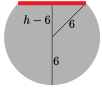
\includegraphics{OE00D_4}
\end{center}
}
At that time, the top surface of the mercury
forms a circular disk of radius $\sqrt{6^2-(h-6)^2}$. (We found this by applying the Pythagorean Theorem to the triangle in the diagram above. In the diagram, $h$ is shown as being larger than 6, but the same equation holds for all $h$ in $[0,12]$.)
Now suppose that in a very short time interval $\dee{t}$, the height
of mercury in the tank changes by $\dee{h}$ (which is negative). Then in this
time interval the amount of the mercury in the tank decreases by
$-\pi\big(\sqrt{6^2-(h-6)^2}\ \big)^2\dee{h}$. (That's the volume of the
red disk in the figure above.) This must be the same as the amount of mercury
that flows through the hole in this time interval. The  mercury comes out of the hole as a cylinder. Its radius is the radius of the hole, $\frac{1}{12}$ foot, and its length is the distance the mercury travels in $\dee{t}$ seconds, $v(t)\dee{t}$ feet. So, the volume of escaped mercury is
 $\pi\big(\frac{1}{12}\big)^2 v\,\dee{t}
=\pi\big(\frac{1}{12}\big)^2 \sqrt{2gh}\,\dee{t}$.
This gives us a separable differential equation.
\begin{align*}
-\pi{\big(\sqrt{6^2-(h-6)^2}\ \big)}^2\dee{h}
    &=\pi\Big(\frac{1}{12}\Big)^2 \sqrt{2gh}\,\dee{t}\\
-{\big({36-(h^2-12h+36)}\ \big)}\dee{h}
    &=\Big(\frac{1}{12}\Big)^2 \sqrt{2gh}\,\dee{t}\\
\big(h^2-12h\big)\dee{h}
    &=\frac{1}{144} \sqrt{2g}\sqrt{h}\,\dee{t}\cr
 \big(h^{3/2}-12h^{1/2}\big)\dee{h}&=\frac{1}{144} \sqrt{2g}\,\dee{t}\cr
\int \big(h^{3/2}-12h^{1/2}\big)\dee{h}&=\int\frac{1}{144} \sqrt{2g}\,\dee{t}\cr
 \frac{h^{5/2}}{5/2}-12\frac{h^{3/2}}{3/2}&=\frac{1}{144} \sqrt{2g}\,t+C
\intertext{At time $0$, the height is $12$, so $C=\frac{12^{5/2}}{5/2}-12\frac{12^{3/2}}{3/2}
=12^{5/2}\big(\frac{2}{5}-\frac{2}{3}\big)
=-\frac{4}{15}12^{5/2}$, which yields}
\frac{h^{5/2}}{5/2}-12\frac{h^{3/2}}{3/2}&=\frac{1}{144} \sqrt{2g}\,t
-\frac{4}{15}12^{5/2}
\intertext{We want to find the time $t$ when the height is $h=0$.}
0&=\frac{1}{144} \sqrt{2g}\,t-\frac{4}{15}12^{5/2}\\
\frac{1}{144} \sqrt{2g}\,t&=\frac{4}{15}12^{5/2}\\
 t&=\frac{4\times 144}{15} \sqrt{\frac{12^5}{2g}}\\
&=38.4 \sqrt{\frac{124416}{g}}\approx 2,394\,\text{sec }\approx 0.665\, \text{hr}
\end{align*}
\end{solution}
%%%%%%%%%%%%%%%%%%%%%%%%%%%%%%%%%%%%%%%%

\begin{question}[2001A]
Consider the equation
\begin{align*}
f(x)=3+\int_0^x\big(f(t)-1\big)\big(f(t)-2\big)\ \dee{t}
\end{align*}
\begin{enumerate}[(a)]
\item
 What is $f(0)$?
\item
Find the differential equation satisfied by $f(x)$.
\item
Solve the initial value problem determined in (a) and (b).
\end{enumerate}

\end{question}

\begin{hint}
The fundamental theorem of calculus will be useful in part (b).
\end{hint}

\begin{answer}
(a) $3$
\qquad (b)   $y'=(y-1)(y-2)$
\qquad (c)  $f(x)=\dfrac{4-e^x}{2-e^x}$
\end{answer}

\begin{solution} (a)
Setting $x=0$ gives
\begin{align*}
f(0)=3+\int_0^0\big(f(t)-1\big)\big(f(t)-2\big)\ \dee{t}= 3
\end{align*}

\noindent (b) By the Fundamental Theorem of Calculus part 1,
\begin{align*}
f'(x)=\diff{}{x}\int_0^x\big(f(t)-1\big)\big(f(t)-2\big)\ \dee{t}
=\big(f(x)-1\big)\big(f(x)-2\big)
\end{align*}
Thus $y=f(x)$ obeys  the differential equation $y'=(y-1)(y-2)$.

\noindent (c) If $y\ne 1,2$,
\begin{align*}
\diff{y}{x}&=(y-1)(y-2) \\
\frac{\dee{y}}{(y-1)(y-2)}&=\dee{x}\\
\int\frac{\dee{y}}{(y-1)(y-2)}&=\int\dee{x}
\intertext{Using the method of partial fractions,}
\int\left(\frac{1}{y-2}-\frac{1}{y-1}\right)\dee{y}&=\int \dee{x} \\
 \log|y-2|-\log|y-1|&=x+C\\
  \log\left|\frac{y-2}{y-1}\right|&=x+C
\intertext{
Observe that $\diff{y}{x}=(y-1)(y-2)>0$ for all $y\ge 2$. That is, $f(x)$
is increasing at all $x$ for which $f(x)>2$. As $f(0)=3$, $f(x)$ increases
for all $x\ge 0$, and $f(x)\ge 3$ for all $x\ge 0$. So we may drop the absolute
value signs.}
\log\frac{f(x)-2}{f(x)-1}&=x+C\\
\frac{f(x)-2}{f(x)-1}&=e^Ce^x
\intertext{
At $x=0$, $\frac{f(x)-2}{f(x)-1}=\frac{1}{2}$ so $e^C=\frac{1}{2}$.}
\frac{f(x)-2}{f(x)-1}&=\frac{1}{2} e^x\\
 2f(x)-4&=[f(x)-1]e^x\\
[2-e^x]f(x)&=4-e^x \\
  f(x)&=\frac{4-e^x}{2-e^x}
\end{align*}

\end{solution}
%%%%%%%%%%%%%%%%%%%%%%%%%%%%%%%%%%%%%%%%

\begin{question}[2002A]

\end{question}
A tank 2 m tall is to be made with circular cross--sections
with radius $r=y^p$. Here $y$ measures the vertical distance from
the bottom of the tank and $p$ is a positive constant to be
determined. You may assume that when the tank drains, it obeys
Torricelli's law, that is
\begin{align*}
A(y)\diff{y}{t}=-c\sqrt{y}
\end{align*}
for some constant $c$ where $A(y)$ is the cross--sectional area of the
tank at height $y$. It is desired that the tank be constructed so
that the top half
($y=2$ to $y=1$) takes exactly the same amount of time to drain as the
bottom half ($y=1$ to $y=0$). Determine the value of $p$ so that the tank
has this property. \emph{Note:} it is not possible or necessary to find
$c$ for this question.
\begin{hint}
For any $p>0$, determine first $y(t)$ (in terms of $p$ and $c$) and then the times (also depending on $p$ and $c$) at which
$y=2$, $y=1$ and $y=0$. The condition that ``the top half
takes exactly the same amount of time to drain as the
bottom half'' then gives an equation that determines $p$.
\end{hint}

\begin{answer}
$p=\frac{1}{4}$
\end{answer}

\begin{solution}
Suppose that at time $t$ (measured in hours starting at, say, noon),
the water in the tank has height $y$, which is
between 0 and 2 metres. At that time, the top surface of the water
forms a circular disk of radius $r=y^p$ and area $A(y)=\pi y^{2p}$.
Thus, by Torricelli's law,
\begin{align*}
\pi y^{2p}\diff{y}{t}&=-c\sqrt{y}\\
-\frac{\pi}{c}\cdot y^{2p-{1\over 2}}\dee{y}&=\,\dee{t}\\
\int-\frac{\pi}{c}\cdot y^{2p-{1\over 2}}\dee{y}&=\,\int \dee{t}\\
 -\frac{\pi}{c}\cdot\frac{y^{2p+{1\over 2}}}{2p+{1\over 2}}+d &=t
\intertext{for some constant $d$. At time $t=0$, the height is $y=2$, so
$d=\displaystyle\frac{\pi}{c}\cdot\frac{2^{2p+{1\over 2}}}{2p+{1\over 2}}$
\ .}
t&=\frac{\pi}{c}\bigg(\frac{2^{2p+{1\over 2}}}{2p+{1\over 2}}
-\frac{y^{2p+{1\over 2}}}{2p+{1\over 2}}\bigg)\\
&=\frac{\pi}{c(2p+\frac12)}\left(2^{2p+\frac12}-y^{2p+\frac12}\right)
\end{align*}
The time at which the height is $1$ is obtained by subbing $y=1$ into this
formula. The time at which the height is $0$ is obtained by subbing $y=0$
into this formula. Thus the condition that the top half
($y=2$ to $y=1$) takes exactly the same amount of time to drain as the
bottom half ($y=1$ to $y=0$) is:
\begin{align*}
t(2)-t(1)&=t(1)-t(0)\\
0-t(1)&=t(1)-t(0)\\
t(0)&=2t(1)\\
\frac{\pi}{c(2p+\frac12)}\left(2^{2p+\frac12}-0^{2p+\frac12}\right)&=
2\frac{\pi}{c(2p+\frac12)}\left(2^{2p+\frac12}-1^{2p+\frac12}\right)\\
2^{2p+\frac12}&=
2\left(2^{2p+\frac12}-1\right)\\
2^{2p+\frac12}&=
2\cdot 2^{2p+\frac12}-2\\
2&=2^{2p+\frac12}\\
1&=2p+\frac12\\
p&=\frac14
\end{align*}

\end{solution}
%%%%%%%%%%%%%%%%%%%%%%%%%%%%%%%%%%%%%%%%





\begin{question}
Suppose $f(t)$ is a continuous, differentiable function and the root mean square of $f(t)$ on $[a,x]$ is equal to the average of $f(t)$ on $[a,x]$ for all $x$. That is,
\begin{equation}
\frac{1}{x-a}\int_a^xf(t)\,\dee(t)=\sqrt{\frac{1}{x-a}\int_a^x f^2(t)\,\dee{t}}\tag{$*$}
\end{equation}
You may assume $x>a$.

\begin{enumerate}[(a)]
\item Guess a function $f(t)$ for which the average of $f(t)$ is the same as the root mean square of $f(t)$ on any interval.
\item Differentiate both sides of the given equation.
\item Simplify your answer from (b) by using Equation~($*$) to replace all terms containing $\int_a^x f^2(t)\,\dee{t}$ with terms containing $\int_a^x f(t)\,\dee{t}$.
\item Let $Y(x) = \int_a^x f(t)\,\dee{t}$, so the equation from (c) becomes a differential equation. Find all functions that satisfy it.
\item What is $f(t)$?
\end{enumerate}
\end{question}
\begin{hint}
For (a), think of a very simple function.

The equation in the question statement is equivalent to the equation
\[\frac{1}{\sqrt{x-a}}\int_a^xf(t)\,\dee(t)=\sqrt{\int_a^x f^2(t)\,\dee{t}}\]
which is, in some cases, easier to use.

For (d), you'll want to let $Y(x)=\int_a^x f(t)\,\dee{t}$, and use the quadratic equation. \end{hint}
\begin{answer}
\begin{enumerate}
\item[(a)] One possible answer: $f(t)=0$
\item[(b)] $\displaystyle \frac{1}{\sqrt{x-a}}\left[f(x) - \frac{1}{2(x-a)}\int_a^x f(t)\,\dee{t}\right]
=\frac{f^2(x)}{2\sqrt{\int_a^xf^2(t)\,\dee{t}}}$
\item[(c)] $\displaystyle \frac{2}{x-a}\int_a^x f(t)\,\dee{t}\left[f(x) - \frac{1}{2(x-a)}\int_a^x f(t)\,\dee{t}\right]=f^2(x)$
\item[(d)] $Y(x) = D(x-a)$, where $D$ is any constant
\item[(e)] $f(t)=D$, for any nonnegative constant $D$
\end{enumerate}
\end{answer}
\begin{solution}
\begin{enumerate}[(a)]
\item If we let $f(t)=0$ for all $t$, then its average over any interval is 0, as is its root mean square.
\item
Let's start by simplifying the given equation.
\begin{align}
\notag \frac{1}{x-a}\int_a^x f(t)\,\dee{t}&=\sqrt{\frac{1}{x-a}\int_a^x f^2(t)\,\dee{t}}\\
\frac{1}{\sqrt{x-a}}\int_a^x f(t)\,\dee{t}&=\sqrt{\int_a^x f^2(t)\,\dee{t}} \label{prob_s2.4:eq.simplified}\\
\color{red}\diff{}{x}\left\{\frac{1}{\sqrt{x-a}}\int_a^x f(t)\,\dee{t}\right\}&=\color{blue}\diff{}{x}\left\{\sqrt{\int_a^x f^2(t)\,\dee{t}}\right\}\label{prob_s2.4:eq.diffbothsides}
\end{align}
For the derivative on the left, we use the product rule and the Fundamental Theorem of Calculus, part 1.
\begin{align*}
\color{red}\diff{}{x}\left\{\frac{1}{\sqrt{x-a}}\int_a^x f(t)\,\dee{t}\right\}&=\diff{}{x}\left\{\frac{1}{\sqrt{x-a}}\right\}\int_a^x f(t)\,\dee{t} + \frac{1}{\sqrt{x-a}}\cdot\diff{}{x}\left\{\int_a^x f(t)\,\dee{t}\right\}\\
&=-\frac{1}{2\sqrt{x-a}^3}\int_a^x f(t)\,\dee{t} + \frac{f(x)}{\sqrt{x-a}}
\\
&=\color{red}\frac{1}{\sqrt{x-a}}\left[f(x) - \frac{1}{2(x-a)}\int_a^x f(t)\,\dee{t}\right]
\intertext{For the derivative on the right in Equation~(\ref{prob_s2.4:eq.diffbothsides}), we use the chain rule and the Fundamental Theorem of Calculus, part 1.}
\color{blue}\diff{}{x}\left\{\sqrt{\int_a^x f^2(t)\,\dee{t}}\right\}&=\frac{1}{2}\left(\int_a^x f^2(t)\,\dee{t}\right)^{-\frac12}\cdot\diff{}{x}\left\{\int_a^x f^2(t)\,\dee{t}\right\}\\
&=\color{blue}\frac{f^2(x)}{2\sqrt{\int_a^xf^2(t)\,\dee{t}}}
\end{align*}
So, Equation~(\ref{prob_s2.4:eq.diffbothsides}) yields the following:
\begin{align}
\color{red}\frac{1}{\sqrt{x-a}}\left[f(x) - \frac{1}{2(x-a)}\int_a^x f(t)\,\dee{t}\right]
&=\color{blue}\frac{f^2(x)}{2\sqrt{\int_a^xf^2(t)\,\dee{t}}}\label{prob_s2.4:b}
\end{align}
\item
From Equation~(\ref{prob_s2.4:eq.simplified}), $\sqrt{\int_a^x f^2(t)\,\dee{t}} = \frac{1}{\sqrt{x-a}}\int_a^x f(t)\,\dee{t}$.
\begin{align*}
\frac{1}{\sqrt{x-a}}\left[f(x) - \frac{1}{2(x-a)}\int_a^x f(t)\,\dee{t}\right]&=\frac{f^2(x)}{2\frac{1}{\sqrt{x-a}}\int_a^x f(t)\,\dee{t}}\\
\frac{2}{x-a}\int_a^x f(t)\,\dee{t}\left[f(x) - \frac{1}{2(x-a)}\int_a^x f(t)\,\dee{t}\right]&=f^2(x)
\end{align*}
\item
Now what we have is a differential equation, although it might not look like it. Let $Y = \int_a^x f(t)\,\dee{t}$. Then $\diff{Y}{x} = f(x)$.
\begin{align}
\frac{2}{x-a}Y\left[\diff{Y}{x} - \frac{1}{2(x-a)}Y\right]&=\left(\diff{Y}{x}\right)^2\label{prob_s2.4:eq.diffeq}\\
\intertext{We're used to solving differential equations of the form $\diff{Y}{x}=$(something). So, let's manipulate our equation until it has this form.}
\notag \left(\diff{Y}{x}\right)^2-\left(\frac{2Y}{x-a}\right)\left(\diff{Y}{x}\right)+\left(\frac{Y}{x-a}\right)^2&=0
\end{align}
This is a quadratic equation, with variable $\diff{Y}{x}$. Its solutions are:
\begin{align}
\notag \diff{Y}{x}&=\frac{\left(\frac{2Y}{x-a}\right)\pm\sqrt{\left(\frac{2Y}{x-a}\right)^2-4\cdot\left(\frac{Y}{x-a}\right)^2}}{2}\\
\notag&=\frac{\frac{2Y}{x-a}\pm 0}{2}\\
\notag&=\frac{Y}{x-a}
\intertext{This gives us the separable differential equation}
\notag\diff{Y}{x}&=\frac{Y}{x-a}  \\
\frac{\dee{Y}}{Y}&=\frac{\dee{x}}{x-a} \label{prob_s2.4:eq.diffeqdivide}\\
\notag\int\frac{\dee{Y}}{Y}&=\int\frac{\dee{x}}{x-a}\\
\notag\log|Y|&=\log|x-a|+C\\
\notag|Y|&=e^{\log(x-a)+C} = (x-a)e^C\\
\notag Y&=D(x-a)
\end{align}
where $D$ is some constant, $e^C$ or $-e^C$. Note this covers all real constants except $D=0$. If $D=0$, then $Y(x)=0$ for all $x$. This function also satisfies Equation~(\ref{prob_s2.4:eq.diffeq}), so indeed, \begin{equation}
Y(x)=D(x-a) \label{prob_s2.4:eq.d}\end{equation} for \emph{any} constant $D$ is the family of equations satisfying our differential equation.

Remark: the reason we ``lost" the solution $Y(x)=0$ is that in Equation~(\ref{prob_s2.4:eq.diffeqdivide}), we divided by $Y$, thus tacitly assuming it was not identically 0.
\item  Remember $Y=\int_a^x f(t)\,\dee{t}$. So, Equation~(\ref{prob_s2.4:eq.d}) tells us:
 \begin{align*}
\int_a^x f(t)\,\dee{t}&=D(x-a)\\
\diff{}{x}\left\{\int_a^x f(t)\,\dee{t}\right\}&=\diff{}{x}\{D(x-a)\}\\
f(x)&=D
\end{align*}
We should check that this function works.
\begin{align*}
f_{\text{avg}} &= \frac{1}{x-a}\int_a^x D\,\dee{t} = \frac{1}{x-a}\Big[Dt\Big]_{t=a}^{t=x} = \frac{Dx-Da}{x-a}=D\\
f_{\text{RMS}} &= \sqrt{\frac{1}{x-a}\int_a^x D^2\,\dee{t}}
=\sqrt{\frac{1}{x-a}\Big[D^2x\Big]_{t=a}^{t=x}}=\sqrt{\frac{D^2x-D^2a}{x-a}}=\sqrt{D^2}=|D|
\end{align*}
So, $f(x)=D$ works only if $D$ is nonnegative.

That is: the only functions whose average matches their root square mean over every interval are constant, nonnegative functions.

Remark: it was step (c) where we introduced the erroneous answer $f(x)=D$, $D<0$ to our solution. In Equation~(\ref{prob_s2.4:b}), $f(x)=D$ is not a solution if $D<0$:
\begin{align*}
\frac{1}{\sqrt{x-a}}\left[f(x) - \frac{1}{2(x-a)}\int_a^x f(t)\,\dee{t}\right]&=\frac{f^2(x)}{2\sqrt{\int_a^x f^2(t)\,\dee{t}}}\\
\frac{1}{\sqrt{x-a}}\left[D - \frac{1}{2(x-a)}\int_a^x D\,\dee{t}\right]&=\frac{D^2}{2\sqrt{\int_a^x D^2\,\dee{t}}}\\
\frac{1}{\sqrt{x-a}}\left[D - \frac{1}{2(x-a)}D(x-a)\right]&=\frac{D^2}{2\sqrt{ D^2(x-a)}}\\
\frac{1}{\sqrt{x-a}}\left[\frac{1}{2}D \right]&=\frac{D^2}{2|D|\sqrt{x-a}}\\
D&=\frac{D^2}{|D|}=|D|
\end{align*}

In (c), we replace $\sqrt{\int_a^x f^2(t)\,\dee{t}}$, which cannot be negative, with $\frac{1}{\sqrt{x-a}}\int_a^x f(t)\,\dee{t}$, which could be negative if $f(t)=D<0$. Indeed, if $f(t)=D$, then
$\sqrt{\int_a^x f^2(t)\,\dee{t}}  = |D|\sqrt{x-a}$, while
$\frac{1}{\sqrt{x-a}}\int_a^x f(t)\,\dee{t}=D\sqrt{x-a}$.
It is at this point that negative functions creep into our solution.
\end{enumerate}
\end{solution}
%%%%%%%%%%%%%%%%%%%




\begin{Mquestion}
Find the function  $y(x)$ such that
\[\ddiff{2}{y}{x}=\frac{2}{y^3}\cdot\diff{y}{x}\]
and if $x=-\frac{1}{16}\log 3$, then $y=1$ and $\diff{y}{x}=3$.

You do not need to solve for $y$ explicitly.
\end{Mquestion}
\begin{hint}
Start by antidifferentiating both sides of the equation with respect to $x$.
\end{hint}
\begin{answer}
$\displaystyle x=\frac{1}{4}\left(y-1+\frac{1}{4}\log\left|\frac{2y-1}{2y+1}\right|\right)
$
\end{answer}
\begin{solution}
We start by antidifferentiating both sides with respect to $x$.
\begin{align*}
\int \left(\ddiff{2}{y}{x}\right)\,\dee{x}&=\int\left(\frac{2}{y^3}\cdot\diff{y}{x}\right)\,\dee{x}
\intertext{The right integral is in exactly the form we would use for a change of variables (substitution) to $y$.}
\diff{y}{x}&=\int\left(\frac{2}{y^3}\right)\,\dee{y} = -\frac{1}{y^2}+C
\intertext{When $y=1$, $\diff{y}{x}=3$.}
3& =-\frac{1}{1}+C\\
C&=4
\intertext{So,}
\diff{y}{x}&=-\frac{1}{y^2}+4
\intertext{
This is a separable differential equation.
}
\diff{y}{x}&=\frac{4y^2-1}{y^2}
\\
\frac{y^2}{4y^2-1}\,\dee{y}&=\dee{x}\\
\int \frac{y^2}{4y^2-1}\,\dee{y}&=\int \dee{x}\tag{$*$}
\end{align*}
We can evaluate the left integral with partial fractions, but because the numerator has the same degree as the denominator, we have to simplify first. We do this by inspection, but you can also use long division.
\begin{align*}
 \frac{y^2}{4y^2-1}&=\frac{\frac{1}{4}(4y^2-1)+\frac{1}{4}}{4y^2-1}\\
 &=\frac{1}{4}\left(1+\frac{1}{4y^2-1}\right)\\
 &=\frac{1}{4}\left(1+\frac{1}{(2y-1)(2y+1)}\right)\\
 &=\frac{1}{4}\left(1+\frac{1/2}{2y-1}-\frac{1/2}{2y+1}\right)
\end{align*}
Now, we return to ($*$).
\begin{align*}
\int \dee{x}&=\int \frac{y^2}{4y^2-1}\,\dee{y}\\
&= \int \frac{1}{4}\left(1+\frac{1/2}{2y-1}-\frac{1/2}{2y+1}\right)\,\dee{y}\\
&= \frac{1}{4}\left(y+\frac{1}{4}\log|2y-1| - \frac{1}{4}\log|2y+1|\right)\\
&= \frac{1}{4}\left(y+\frac{1}{4}\log\left|\frac{2y-1}{2y+1}\right|\right)\\
x+C&=\frac{1}{4}\left(y+\frac{1}{4}\log\left|\frac{2y-1}{2y+1}\right|\right)
\intertext{When $x=-\frac{1}{16}\log 3$, $y=1$.}
-\frac{1}{16}\log 3 +C &=\frac{1}{4}\left(1+\frac14\log\left| \frac{2-1}{2+1}\right|\right) = \frac{1}{4}+\frac{1}{16}\log\frac{1}{3}\\
C&=\frac{1}{4}
\intertext{So,}
x+\frac{1}{4}&=\frac{1}{4}\left(y+\frac{1}{4}\log\left|\frac{2y-1}{2y+1}\right|\right)\\
x&=\frac{1}{4}\left(y-1+\frac{1}{4}\log\left|\frac{2y-1}{2y+1}\right|\right)
\end{align*}
We can check our answer by differentiating with respect to $x$.
\begin{align*}
x&=\frac{1}{4}\left(y-1+\frac{1}{4}\log\left|\frac{2y-1}{2y+1}\right|\right)\\
4x&=y-1+\frac{1}{4}\log|2y-1| -\frac{1}{4}\log|2y+1|\\
\diff{}{x}\{4x\}&=\diff{}{x}\left\{y-1+\frac{1}{4}\log|2y-1| -\frac{1}{4}\log|2y+1|\right\}\\
4&=\diff{y}{x}+\frac{1}{4}\cdot\frac{2\diff{y}{x}}{2y-1} - \frac{1}{4}\cdot\frac{2\diff{y}{x}}{2y+1}\\
4&=\diff{y}{x}\left(1+\frac{1/2}{2y-1} - \frac{1/2}{2y+1}\right) = \diff{y}{x}\left(\frac{4y^2}{4y^2-1}\right)\\
\diff{y}{x}&=\frac{4y^2-1}{y^2}=4-\frac{1}{y^2} \tag{$**$}
\intertext{Differentiating with respect to $x$ again, using the chain rule,}
\ddiff{2}{y}{x}&=\frac{2}{y^3}\cdot\diff{y}{x}
\end{align*}
This is exactly the differential equation we were meant to solve.
\end{solution}
%%%%%%%%%%%%%%%%%%%
